% LaTeX template for a short report (written for MSES scenario modelling)
% uses LaTeX documentclass "article" for use of sections (not chapter) and References (not Bibliography)
% for Chapters and Bibliography use "documentclass "report
\documentclass[10pt]{article}   % Use article class with 10pt letter
%\documentclass[10pt]{report}
\usepackage[utf8]{inputenc}

%\usepackage[T1]{fontenc}  % 8-bit encoding, helps hyphenation of accented characters -
% https://tex.stackexchange.com/a/677/42066

% Use A4 paper and set margins:
%\usepackage[a4paper, twoside, top=2.0cm, left=3.0cm, bottom=2.0cm, right=2.0cm]{geometry}
\usepackage[a4paper, twoside, top=2.0cm, left=2.0cm, bottom=2.0cm, right=2.0cm]{geometry}
%\usepackage[a4paper, top=2.5cm, left=2.5cm, bottom=2.5cm, right=2.5cm]{geometry}

\usepackage[english]{babel}  % Hyphenation and more for English

\usepackage{pgf}      % Include graphics inside figures using \pgfimage
\usepackage[font=small, labelfont=bf]{caption}  % Stylize figure, table, etc. captions

\usepackage{parskip}         % Replace paragraph indentations with white lines
\usepackage[hyphens]{url}    % Take care of urls, e.g. wrapping in the Bibliography (hyphens: also break at -)

\usepackage{xspace}   % \xspace saves the user from having to type \  or {} after a macro name in text.

% Use the appendix package for nicer appendices:
%\usepackage[toc,page]{appendix}  % MvdS
\usepackage[titletoc]{appendix}
%\usepackage[toc,page,title]{appendix}  % Use \begin{appendices} ... \end{} iso \appendix

% \usepackage[numbib,numindex]{tocbibind}  % Add ToC, List of Figures/Tables/Code listings, Bibliography and Index to ToC
% \usepackage[]{tocbibind}       % Add ToC, List of Figures/Tables/Code listings, Bibliography and Index to ToC
\usepackage[nottoc]{tocbibind}   % ToC without extra "Contents" entry...

\usepackage{amsmath,amssymb,bbm}
\usepackage{enumerate}         % Choose alternative numberings, e.g. \begin{enumerate}[a.]

\usepackage{listings}          % Code listings
\usepackage[section, above, below]{placeins}  % \FloatBarrier - flush floats before \section by default
% \usepackage{pgf}               % Figures

\usepackage{color}
\definecolor{lightgrey}{rgb}{0.9,0.9,0.9}
\definecolor{darkgreen}{rgb}{0.0,0.6,0.0}

% Citations:

% option1: use natbib/bibtex with MvdS_number_url.bst
%\usepackage[numbers, square]{natbib}  % Use numbered citations with square brackets
%\bibliographystyle{MvdS_number_url}  % Use [1], print url = field  (plain doesn't print urls)

%option2: use biblatex/biber without *.bst file
\usepackage[backend=biber, style=numeric, citestyle=numeric-comp, sorting=none]{biblatex} 
\setlength\bibitemsep{0.5\baselineskip}
\usepackage{csquotes}

% \bibliography{mybibliography} % old-style for backward comp. in preamble for biblatex/bibtex
\addbibresource{mybibliography.bib}  % new syntax for BibLaTeX


\usepackage{fancybox}  % Use \ovalbox for key strokes

\newcommand{\ldf}{\usefont{OT1}{cmr}{m}{n}}     % Select default LaTeX font - Computer Modern Roman
%\newcommand{\ldf}{\usefont{OT1}{cmss}{m}{n}}     % Select default LaTeX font - Computer Modern Sans
%\newcommand{\ldf}{\usefont{OT1}{phv}{m}{n}}     % Select default LaTeX font - Helvetica
\newcommand{\ttbf}{\usefont{OT1}{lmtt}{bx}{n}}  % Select bold typewriter font

%\usepackage[font=sf]{caption}  % Use sans-serif font for float captions - not exactly Helvetica



\newcommand{\note}[1]{\color{red}\textbf{#1}\color{black}\xspace}
\newcommand{\marc}[1]{\color{red}\textbf{Marc: #1}\color{black}\xspace}

\newcommand{\myChapter}[1]{
  \chapter{#1}
  \minitoc  % Create a ToC of this chapter
}


% General expressions:
\newcommand{\eg}{\emph{e.g.}\xspace}
\newcommand{\ie}{\emph{i.e.}\xspace}
\newcommand{\etc}{\emph{et cetera}\xspace}
\newcommand{\ff}{\emph{ff}\xspace}

% CLI symbols:
\newcommand{\pipe}{$|$}      % Needed to avoid | in \index{}
\newcommand{\logor}{$|\,|$}  % Needed to avoid | in \index{}
\newcommand{\home}{\url{~}}  % Home directory


% Often used code names:
\newcommand{\NULL}{\code{NULL}}
\newcommand{\void}{\code{void}}
\newcommand{\stdout}{\code{stdout}}
\newcommand{\stderr}{\code{stderr}}

% Man pages:
\newcommand{\man}[2]{\texttt{man #1 #2}\xspace}
\newcommand{\mancmd}[1]{\texttt{man #1}\xspace}

% Code:
\newcommand{\prototype}[3]{\hspace*{2em}\texttt{#1} {\ttbf #2\ldf}(\texttt{#3});\xspace}  % function prototype
\newcommand{\var}[2]{\hspace*{2em}\texttt{#1} {\ttbf #2\ldf};\xspace}  % variable declaration
\newcommand{\code}[1]{\texttt{#1}\xspace}  % inline code
\newcommand{\codeb}[1]{\ttbf #1\ldf\xspace}  % inline bold code
\newcommand{\codeline}[1]{\hspace*{2em}\texttt{#1}}  % separate code line

\newcommand{\cli}[1]{\noindent\hspace*{2em}\code{\$ #1}}  % command line input
\newcommand{\clir}[1]{\noindent\hspace*{2em}\code{\# #1}}  % command line input root
\newcommand{\clo}[1]{\noindent\hspace*{2em}\code{#1}}  % command line output
\newcommand{\clitem}[1]{\item[\code{\$}] \code{#1}}  % cli in itemized list, with $ as bullet
\newcommand{\clitemb}[1]{\item[\codeb{\$}] \codeb{#1}}  % cli in itemized list, with $ as bullet - bold

\newcommand{\key}[1]{\Ovalbox{\texttt{#1}}\xspace}  % key press/combination
\newcommand{\keyb}[1]{\Ovalbox{\ttbf #1\ldf}\xspace}  % key press/combination bold


% Heat pumps
\newcommand{\COP}{\mathrm{COP}}  % COP in "math mode"
\newcommand{\COPh}{\COP_{\mathrm{heating}}}  % COP_heating in "math mode"

\newcommand{\Qh}{Q_{\mathrm{H}}}
\newcommand{\Qc}{Q_{\mathrm{C}}}
\newcommand{\Th}{T_{\mathrm{H}}}
\newcommand{\Tc}{T_{\mathrm{C}}}

\newcommand{\Tin}{T_{\mathrm{in}}}
\newcommand{\Tout}{T_{\mathrm{out}}}

\newcommand{\Ph}{P_{\mathrm{heat}}}
\newcommand{\Pheat}{P_{\mathrm{heat}}}
\newcommand{\Pc}{P_{\mathrm{cool}}}
\newcommand{\Pcool}{P_{\mathrm{cool}}}
\newcommand{\Pel}{P_{\mathrm{el}}}

\newcommand{\degr}{^\circ}
\newcommand{\tdeg}{$\degr$\xspace}
\newcommand{\degC}{\degr\mathrm{C}}
\newcommand{\tdegC}{$\degC$\xspace}

  % Custom commands

\usepackage[pdftex]{hyperref}
\hypersetup{
  colorlinks = true,  % They get a red box around them if false, better set colour to black?
  linkcolor = blue,
  filecolor = magenta,
  citecolor = blue,
  urlcolor = blue,
  % linkcolor = black,
  % citecolor = black,
  % urlcolor = black,
  pdftitle = House Model References,
  pdfauthor = Trung Nguyen,
  pdfsubject = House Models,
  pdfkeywords = house - models - Python,
  pdfcreator = TeXStudio pdfLaTeX2 on Windows,
  pdfproducer = TeXStudio pdfLaTeX2 on Windows,
  bookmarksnumbered = true,  % Number sections in PDF toc
}

\usepackage[onehalfspacing]{setspace}
\usepackage{float}

\usepackage{graphicx}
\usepackage{multirow}

%\renewcommand{\thesection}{\arabic{section}}  % needed for documentclass "report" with sections





%Document title, author and date (empty)
\title{House Model Reference Manual \\
	FutureFactory}
\author{Trung Nguyen, Maarten van den Berg \\
	Marijn Jongerden, Paul van Kan and Rob ter Steeg \\ \\
	Academy of Engineering and Automotive Science (AEA) \\
HAN University of Applied Sciences\\
Arnhem, The Netherlands}
% \date{}

\begin{document}
	
\ldf          % LaTeX default font

% Set up code listing style:
\lstset{
	language=Python,
	% Fonts:
	basicstyle=\ttfamily\footnotesize,
	%keywordstyle=\ttfamily,
	%identifierstyle=,
	%commentstyle=\ttfamily\scriptsize,
	% B/W code:
	% commentstyle=\ttfamily\itshape,  % Italic
	% stringstyle=\ttfamily,
	% identifierstyle=\ttbf,           % Bold typewriter type
	% keywordstyle=\ttbf,              % Bold tt
	% Colour:
	commentstyle=\scriptsize\ttfamily\color{brown},
	stringstyle=\ttfamily\color{darkgreen},
	identifierstyle=\color{blue},
	keywordstyle=\ttfamily\color{red},
	% Spaces:
	showstringspaces=false,
	breaklines=true,
	breakatwhitespace=true,
	% Line numbering:
	numbers=left,
	numberstyle=\tiny,
	stepnumber=2, 
	numbersep=5pt,
	% Frames:
	frame=single,
	frameround=tttt,
	backgroundcolor=\color{lightgrey},
	morekeywords={pthread_create},
}

%\renewcommand{\thelstlisting}{\thechapter.\arabic{lstlisting}}  % This is the default?
%\numberwithin{lstlisting}{section}  % AMSmath: number code listings per section
%\numberwithin{lstlisting}{chapter}  % AMSmath: number code listings per chapter

\maketitle
% \newpage

%\begin{center}
%	\today
%\end{center}

\tableofcontents
\newpage

% \chapter{Introduction}

\section{Introduction}

The report give an overview and compare between the available  PID and advance python control packages. The different PID forms will be discussed in section 2. In section 3 and 4 are the most used PID python packages in practice with their advantages and disadvantages. Finally section 5 give an overview on some advance control and optimization python library.


\newpage

\section{White box lumped model: RC network}
\subsection{White box lumped model}

The objective of the house model for this project is to serve as test environment for a heat pump model, which means that the house model is intended as a tool to help taking building systems design decisions. The house heating demand calculation model implemented for this project is a white box \emph{lumped} model. Specifically, it is a RC network model consisting of resistances (R) and capacities (C). The RC network model is based on the analogy with electrical circuits. The simulation of thermodynamic systems characterizing building elements as resistances or capacities allows to simplify the model while maintaining a high simulation results accuracy \textbf{(Bagheri et al.\cite{en11040890}, Bacher et al\cite{Bacher}.)}.  

There are several types of RC models, the most common being 3R4C models and 3R2C models which are applied on the outer and internal wall. For the simulation of simple house buildings 3R2C models perform as accurate as more complex 3R4C models \textbf{(Fraisse et al.\cite{Fraisse})}. Considering that one of the objectives for this project is to obtain a fast but accurate simulation of a simple dwelling the 3R2C network model appeared a good starting point. In the 3R2C model two indoor temperature nodes are present in the dwelling. \textbf{with capacities (usually an air and a wall temperature) and a well-known outdoor temperature }. \textbf{Between these 3 temperature nodes 3 heat transfer resistances are present. However, the direct heat transfer between the inner walls and the outdoor air is low. Moreover, uncertainties are present about heat transfer coefficients between walls and indoor air, different indoor temperatures in the house rooms and the ground temperature which deviates from the outdoor temperature. In addition, occupancy behaviour varies strongly. }For that reason, we have made a further simplification to a 2R2C model. In section 4 it is shown that this dwelling model delivers a reliable annual energy consumption.


\subsection{House Model R and C Values}

This section presents the basic information for calculating a house model based on an RC network. This category of house models, analogous to electrical impedance networks, may have different numbers of R and C components and may have various component topologies. For the specific model properties, references will be given.

In heat transfer theory the basic thermal circuit contains thermal resistances. Heat transfer occurs via conduction, convection and radiation. In analogy with Ohm's Law for electricity, expressions can be derived for the heat transfer rate (analogous to electrical current) and the thermal resistances (analogous to ohmic resistances) in these three modes of heat transfer. The temperature difference plays a role analogous to the electrical voltage difference. These expressions are shown in Fig.\ref{table_1}.
\begin{figure}[H]
	\centering
	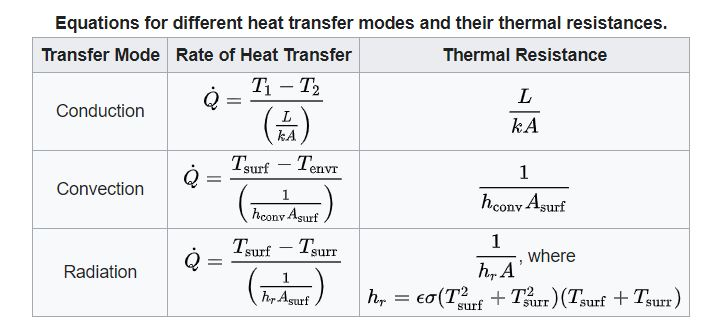
\includegraphics[width=0.8\columnwidth]{Pictures/heat transfer mode.JPG}
	\caption[Short title]{Heat transfer modes\cite{GIGO}}
	\label{table_1}
\end{figure}
\newpage

In \cite{HTTHERMO} and \cite{FUND} the expressions in Fig.\ref{table_1} are derived.
For conduction, the expression for absolute thermal resistance is:  

\begin{equation}
	R = \frac{L}{kA} \qquad \left[ \frac{K}{W} \right]
\end{equation}

\begin{itemize}
    \item $L$ is the distance over which heat transfer takes place, or the thickness of the material $[m]$.
    \item $k$ (also denoted with $\lambda$) is the thermal conductivity of the material. [$\frac{W}{mK}$]. 
    \item $A$ is the conductive surface area  $[m^2]$.
    \item Thermal resistivity is the reciprocal of thermal conductivity and can be expressed as $r =\frac{1}{k}$  in $[\frac{mK}{W}]$

\end{itemize}


For convection and radiation the expression for thermal resistance is: $R = \frac{1}{h \cdot A}$ [$\frac{K}{W}$].

\begin{itemize}
    \item $A$ is the surface area where the heat transfer takes place $[m^2]$.
    \item $h$ is the heat transfer coefficient  [$\frac{W}{m^2K}$]
\end{itemize}


The $R$-value (in Dutch: $R$-waarde or $R_d$-waarde) of a building material \cite{Rvalues_insulation} is the thermal resistance of a square meter surface.
It can be calculated by multiplying the thermal \emph{resistivity} with the thickness of the material in  $m$.
Alternatively it is calculated by dividing the material thickness by the thermal \emph{conductivity} $k$ or $\lambda$.

\begin{equation}
	\text{R-value} = r \cdot L  \qquad \text{or} \qquad  \text{R-value} = \frac{L}{k}  \qquad \text{or} \qquad  
	\text{R-value} = \frac{L}{\lambda}  \qquad \left[m \cdot \frac{m \cdot K}{W} \right] = \left[\frac{m^2 \cdot K}{W}\right] 
\end{equation}


Some typical heat transfer $R$-values are: \cite{OVERALL}: 

\begin{itemize}
	\item Static layer of air, 40 mm thickness (1.57 in)  : R = 0.18 [$\frac{m^2K}{W}$].
	\item Inside heat transfer resistance, horizontal current : R = 0.13 [$\frac{m^2K}{W}$]. 
	\item Outside heat transfer resistance, horizontal current : R = 0.04 [$\frac{m^2K}{W}$].
	\item Inside heat transfer resistance, heat current from down upwards : R = 0.10 [$\frac{m^2K}{W}$].
	\item Outside heat transfer resistance, heat current from above downwards : R = 0.17 [$\frac{m^2K}{W}$].
\end{itemize}


\textbf{Note}: in Dutch building physics, $R$-values with subscripts are used:
\begin{itemize}
	\item $R_d$-waarde is used for the $R$-value of a homogeneous building material. $ R = \frac{L}{\lambda} $
	\item $R_c$-waarde (compound, construction) is used for the $R$-value of a surface consisting of several building materials. $R_c$-waarden are calculated as the surface-area weighted sum of $R_d$-waarden of the building materials. 
	For the simplest roof surface, $R_c$ is a linear combination of the $R$-values of the wooden joists and girders (spanten en gordingen) and the areas in between with a certain insulation material sandwich.
	The $R$-value of the insulation sandwich, in its turn, is the sum of the $R$-values of the materials in the sandwich. From inside out, this sandwich may consist of \textit{e.g.} a 9.5 mm plaster board, a PIR/PUR insulation panel, an air gap and a wooden roof deck. All types of $R$-value have the dimension $ [\frac{m^2 \cdot K}{W}] $.
\end{itemize}

\begin{figure}[H]
	\centering
	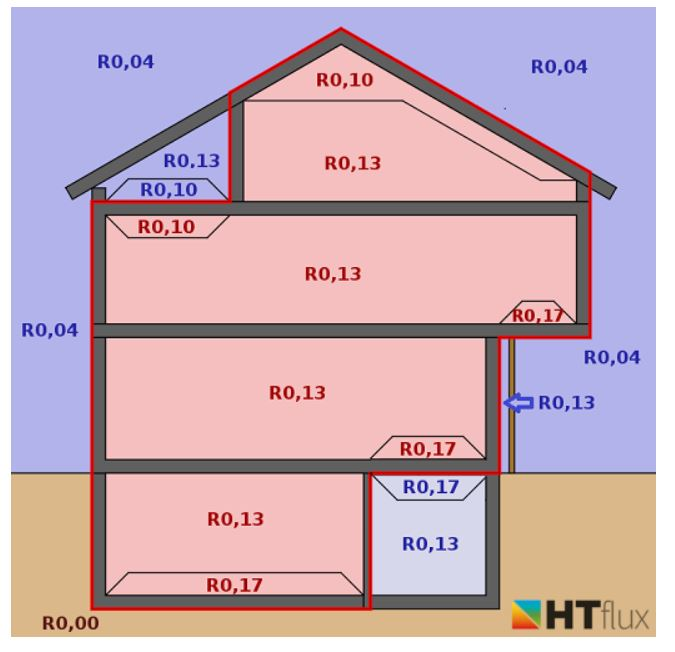
\includegraphics[width=0.8\columnwidth]{Pictures/Overview of heat resistances.JPG}
	\caption[Short title]{An overview of $R$-values for heat transfer \cite{SURFREST}.}
	\label{fig:overview}
\end{figure}


The standard R\textsubscript{c}-values that have been used for facades, roof and floor until 2020 are summarized in Fig.\ref{fig:Rcvalues}:

\begin{figure}[H]
	\centering
	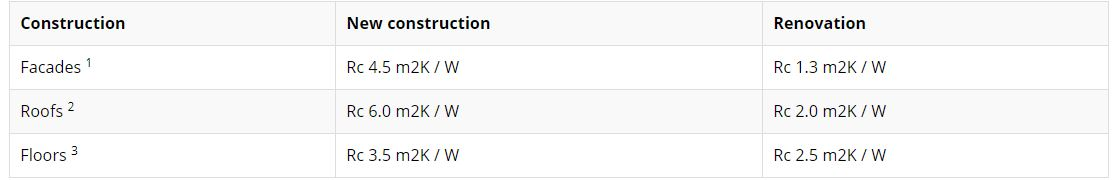
\includegraphics[width=1.0\columnwidth]{Pictures/Rc_values_2020.JPG}
	\caption[Short title]{R\textsubscript{c} Values \cite{ISOL}}
	\label{fig:Rcvalues}
\end{figure}

New standard values will be used from 1-1-2021, since the building standard NEN 1068 will be replaced by the NTA 8800 standard. The old and new situation is described in "EnergieVademecum Energiebewust ontwerpen van nieuwbouwwoningen", Hoofdstuk 5: Thermische isolatie, thermische bruggen en luchtdichtheid.
\cite{ISSO}.

\begin{figure}[H]
	\centering
	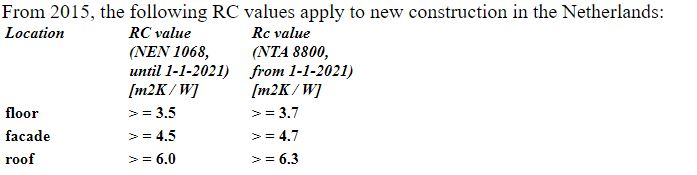
\includegraphics[width=1.0\columnwidth]{Pictures/Rc_values_2021.JPG}
	\caption[Short title]{R\textsubscript{c} Values \cite{RVALUE}}
	\label{fig:newRc}
\end{figure}

The values used for different types of houses such as: row houses, detached houses and apartments can be found in the document "Voorbeeldwoningen 2011" \cite{VOORBEELD}. An example with values for a common type of row house, built in the period from 1975 to 1991 is shown in Fig. \ref{row_house}:


\begin{figure}[H]
	\centering
	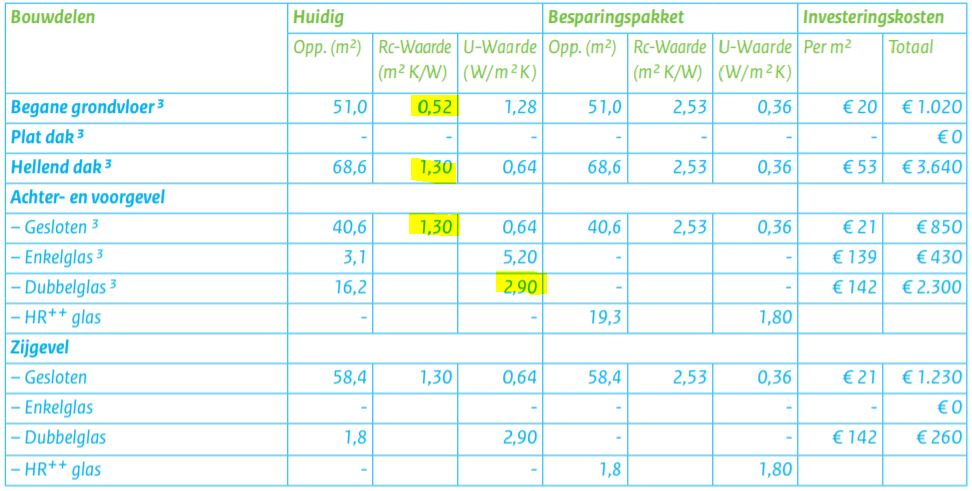
\includegraphics[width=0.8\columnwidth]{Pictures/row_house_1975-1991.JPG}
	\caption[Short title]{R\textsubscript{c}-values for a row house type built between 1975-1991 \cite{VOORBEELD}}
	\label{row_house}
\end{figure} 
\newpage

\subsection{Dwelling (envelope) model analogous to a 2R-2C network}

The heat flow will be modelled by analogy to an electrical circuit where heat transfer rate is analogous to by current, temperature difference is analogous to potential difference, heat sources are represented by constant current sources, absolute thermal resistances are represented by resistors and \textbf{thermal capacitance} heat capacity ? by capacitors \cite{AbsTR}. Figure \ref{fig:Analogies} summarizes the similar term use in different fields.

\begin{figure}[H]
	\centering
	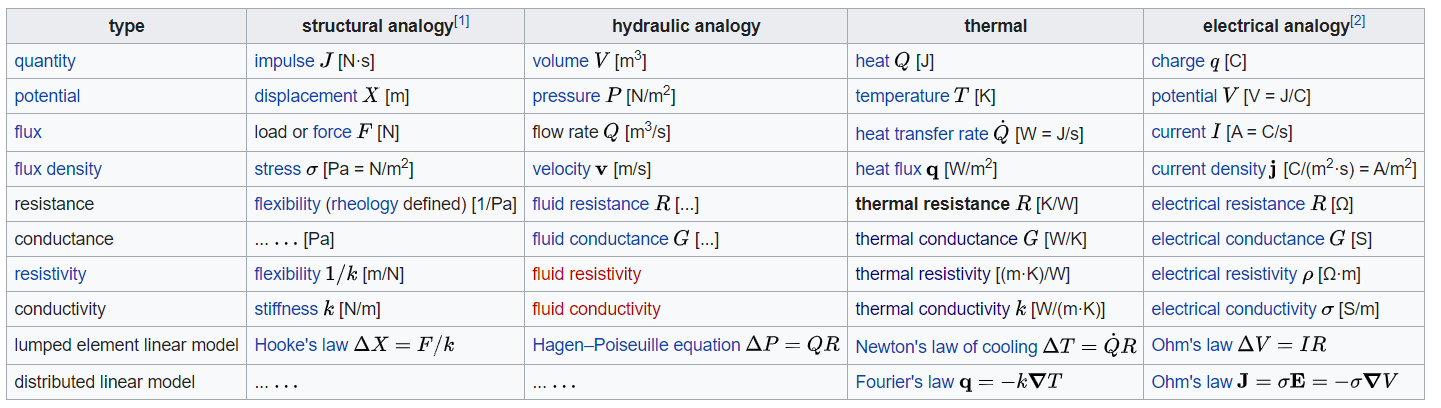
\includegraphics[width=1.0\columnwidth]{Pictures/Analogies.png}
	\caption[Short title]{Table of Analogies  \cite{AbsTR}}
	\label{fig:Analogies}
	\end{figure} 

The 2R-2C house model structure is implemented as described below. The schematic of an envelope house model has been shown in figure  \ref{fig:envelope2R2C} and the equivalent electrical 2R-2C network with components and topology is given in fig  \ref{fig:elec2R2C}.

\begin{figure}[H]
	\centering
	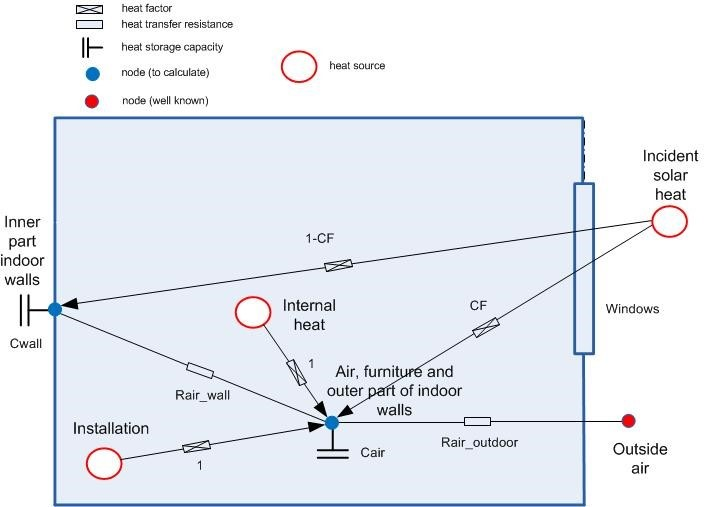
\includegraphics[width=1.0\columnwidth]{Pictures/envelopRC.jpg}
	\caption[Short title]{Schematic of envelope model}
	\label{fig:envelope2R2C}
	\end{figure} 
	

\begin{figure}[H]
	\centering
	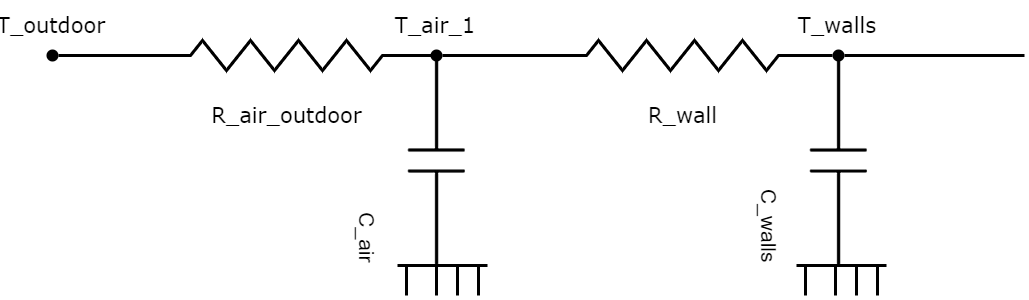
\includegraphics[width=1.0\columnwidth]{Pictures/2R2C_Model.png}
	\caption[Short title]{2R-2C house model}
	\label{fig:elec2R2C}
	\end{figure}
	
The model consists of two heat capacities C\textsubscript{air, indoor} and C\textsubscript{wall} and two resistances R\textsubscript{wall} and R\textsubscript{air, outdoor}. The incident solar energy is divided between C\textsubscript{wall} and C\textsubscript{air} through the convection factor CF. It is assumed that both internal heat (lighting, occupancy and electric devices) and supplied heat (installation) initially heat up the indoor air. In Fig. \ref{fig:envelope2R2C}, they are fully released at the T\textsubscript{air} node. 

 It is also assumed that furniture and the \textbf{surface part} of the walls have the same temperature as the air \textbf{and the wall mass is divided between the air and wall mass}. Thus, the heat capacity of the air node consists of the air heat capacity, furniture heat capacity and the heat capacity \textbf{of a part of the walls}. \textbf{Appendix A} presents the coefficients in the dwelling model. In the resistance R\textsubscript{air, outdoor} the influence of heat transmission through the outdoor walls and natural ventilation is considered. 
 
For the air and wall nodes the following power balances can be set up: 

\begin{equation}
C_{air}\frac{dT_{air}}{dt}=\frac{T_{outdoor}-T_{air}}{R_{air_{\_}outdoor}} + \frac{T_{wall}-T_{air}}{R_{air_{\_}wall}} + \dot{Q}_{inst} + \dot{Q}_{internal} + CF\cdot\dot{Q}_{solar}
\end{equation}

\begin{equation}
C_{wall}\frac{dT_{wall}}{dt}=\frac{T_{air}-T_{wall}}{R_{air_{\_}wall}} + (1-CF)\cdot\dot{Q}_{solar}
\end{equation}


 \begin{itemize}
      \item $CF$: convection factor (solar radiation): the convection factor is the part of the solar radiation that enters the room and is released directly convectively into the room.
      \item $\dot{Q}_{inst}$: delivered heat from heating system (radiator) [W].
      \item $\dot{Q}_{inernal}$: internal heat [W].
      \item $\dot{Q}_{solar}$: heat from solar irradiation [W].
      \item $T_{air}$: indoor air temperature $^o$C.
      \item $T_{outdoor}$: outdoor temperature $^o$C.
      \item $T_{wall}$: wall temperature $^o$C.
      \item $R_{air_{\_}wall}$: walls surface resistance [$\frac{K}{W}$].
      \item $R_{air_{\_}outdoor}$: outdoor surface resistance [$\frac{K}{W}$].
      \item $C_{air}$: air thermal capacitance (heat capacity) [$\frac{J}{K}$]\cite{Thermalmass}.
      \item $C_{wall}$: wall thermal capacitance (heat capacity) [$\frac{J}{K}$]\cite{Thermalmass}.
    \end{itemize}

\newpage   

Total heat transfer of solar irradiation through the glass windows. 
\begin{equation}
\dot{Q}_{solar}=g.\sum(A_{glass}.\dot{q}_{solar})
\end{equation}

\begin{itemize}
    \item $\dot{q}_{solar}$: solar radiation on the outdoor walls [$\frac{W}{m^2}$]. 
    \item g: g value of the glass (ZTA in dutch) [0..1]\cite{zontoetreding}
    \item A: glass surface [$m^2$].
\end{itemize}

%7.6.6.1.2 Ramen met niet-verstrooiende beglazing NTA8800
%https://help.dgmr.nl/bink9/zontoetredingsfactor-zta.html
%https://www.joostdevree.nl/shtmls/zta.shtml
%ISSO-Handboek Zonnestraling: 5.5.1 en 5.2


\newpage

\section{Dwelling (envelope) model analogous to a 2R-2C network}

The 2R-2C house model structure is implemented as described below:
	
\begin{figure}[H]
	\centering
	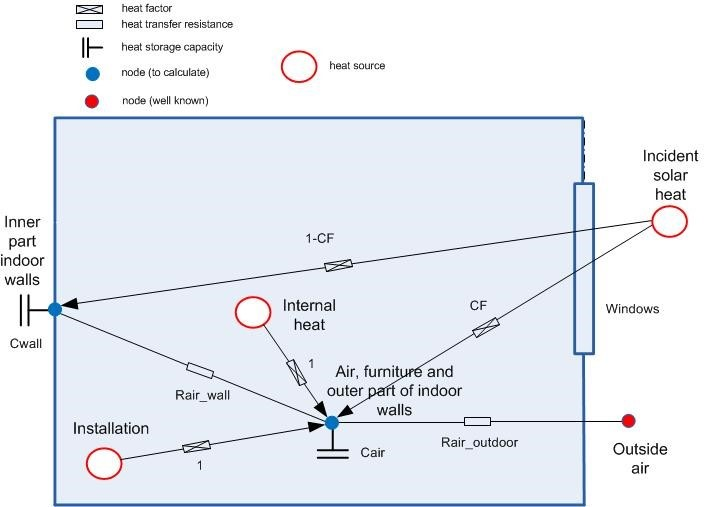
\includegraphics[width=1.0\columnwidth]{Pictures/envelopRC.jpg}
	\caption[Short title]{Schematic of envelope model}
	\label{fig:envelope2R2C}
	\end{figure} 
	
The equivalent electrical 2R-2C network with components and topology is given in Fig. \ref{fig:elec2R2C}.

\begin{figure}[H]
	\centering
	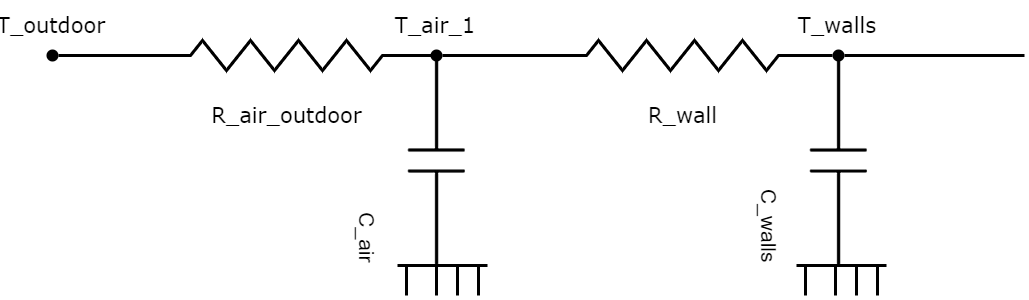
\includegraphics[width=1.0\columnwidth]{Pictures/2R2C_Model.png}
	\caption[Short title]{2R-2C house model}
	\label{fig:elec2R2C}
	\end{figure}
	
The model consists of two capacitances C\textsubscript{air, indoor} and C\textsubscript{wall} and two resistances R\textsubscript{wall} and R\textsubscript{air, outdoor}. The incident solar energy is divided between C\textsubscript{wall} and C\textsubscript{air} through the convection factor CF. It is assumed that both internal heat (lighting, occupancy and electric devices) and supplied heat (installation) initially heat up the indoor air. In Fig. \ref{fig:elec2R2C}, they are fully released at the T\textsubscript{air} node. 

 It is also assumed that furniture and the surface part of the walls have the same temperature as the air and the wall mass is divided between the air and wall mass. Thus, the capacity of the air node consists of the air capacity, furniture capacity and capacity of a part of the walls. \textbf{Appendix A} presents the coefficients in the dwelling model. In the resistance R\textsubscript{air, outdoor} the influence of heat transmission through the outdoor walls and natural ventilation is considered. 
 
For the air and wall nodes the following energy balances can be set up: 

\begin{equation}
C_{air}\frac{dT_{air}}{dt}=\frac{T_{outdoor}-T_{air}}{R_{air_{\_}outdoor}} + \frac{T_{wall}-T_{air}}{R_{air_{\_}wall}} + \dot{Q}_{inst} + \dot{Q}_{internal} + CF\cdot\dot{Q}_{solar}
\end{equation}

\begin{equation}
C_{wall}\frac{dT_{wall}}{dt}=\frac{T_{air}-T_{wall}}{R_{air_{\_}wall}} + (1-CF)\cdot\dot{Q}_{solar}
\end{equation}

 \begin{itemize}
      \item CF: Convection factor (solar radiation): the convection factor is the part of the solar radiation that enters the room and is released directly convectively into the room
      \item $\dot{Q}_{inst}$: delivered heat from heating system (radiator) [W].
      \item $\dot{Q}_{solar}$: heat from solar irradiation [W].
      \item $T_{air}$: indoor air temperature $^o$C.
      \item $T_{outdoor}$: outdoor temperature $^o$C.
      \item $T_{wall}$: wall temperature $^o$C.
      \item $R_{air_{\_}wall}$: walls surface resistance [$\frac{K}{W}$].
      \item $R_{air_{\_}outdoor}$: outdoor surface resistance [$\frac{K}{W}$].
      \item $C_{air}$: air capacity [$\frac{J}{K}$].
      \item $C_{wall}$: wall capacity [$\frac{J}{K}$].
    \end{itemize}
    

Total heat transfer of solar irradiation through the glass windows. 
\begin{equation}
Q_{solar}=g.\sum(A_{glass}.q_{solar})
\end{equation}

\begin{itemize}
    \item $q_{solar}$: solar radiation on the outdoor walls [$\frac{W}{m^2}$]. 
    \item g: g value of the glass (ZTA in dutch) [0..1]\cite{zontoetreding}
    \item A: glass surface [$m^2$].
\end{itemize}

%7.6.6.1.2 Ramen met niet-verstrooiende beglazing NTA8800
%https://help.dgmr.nl/bink9/zontoetredingsfactor-zta.html
%https://www.joostdevree.nl/shtmls/zta.shtml
%ISSO-Handboek Zonnestraling: 5.5.1 en 5.2

\newpage
\chapter{2 Zones house model 7R4C network}

The 4R-7C house model structure is implemented as described below:
	
\begin{figure}[H]
	\centering
	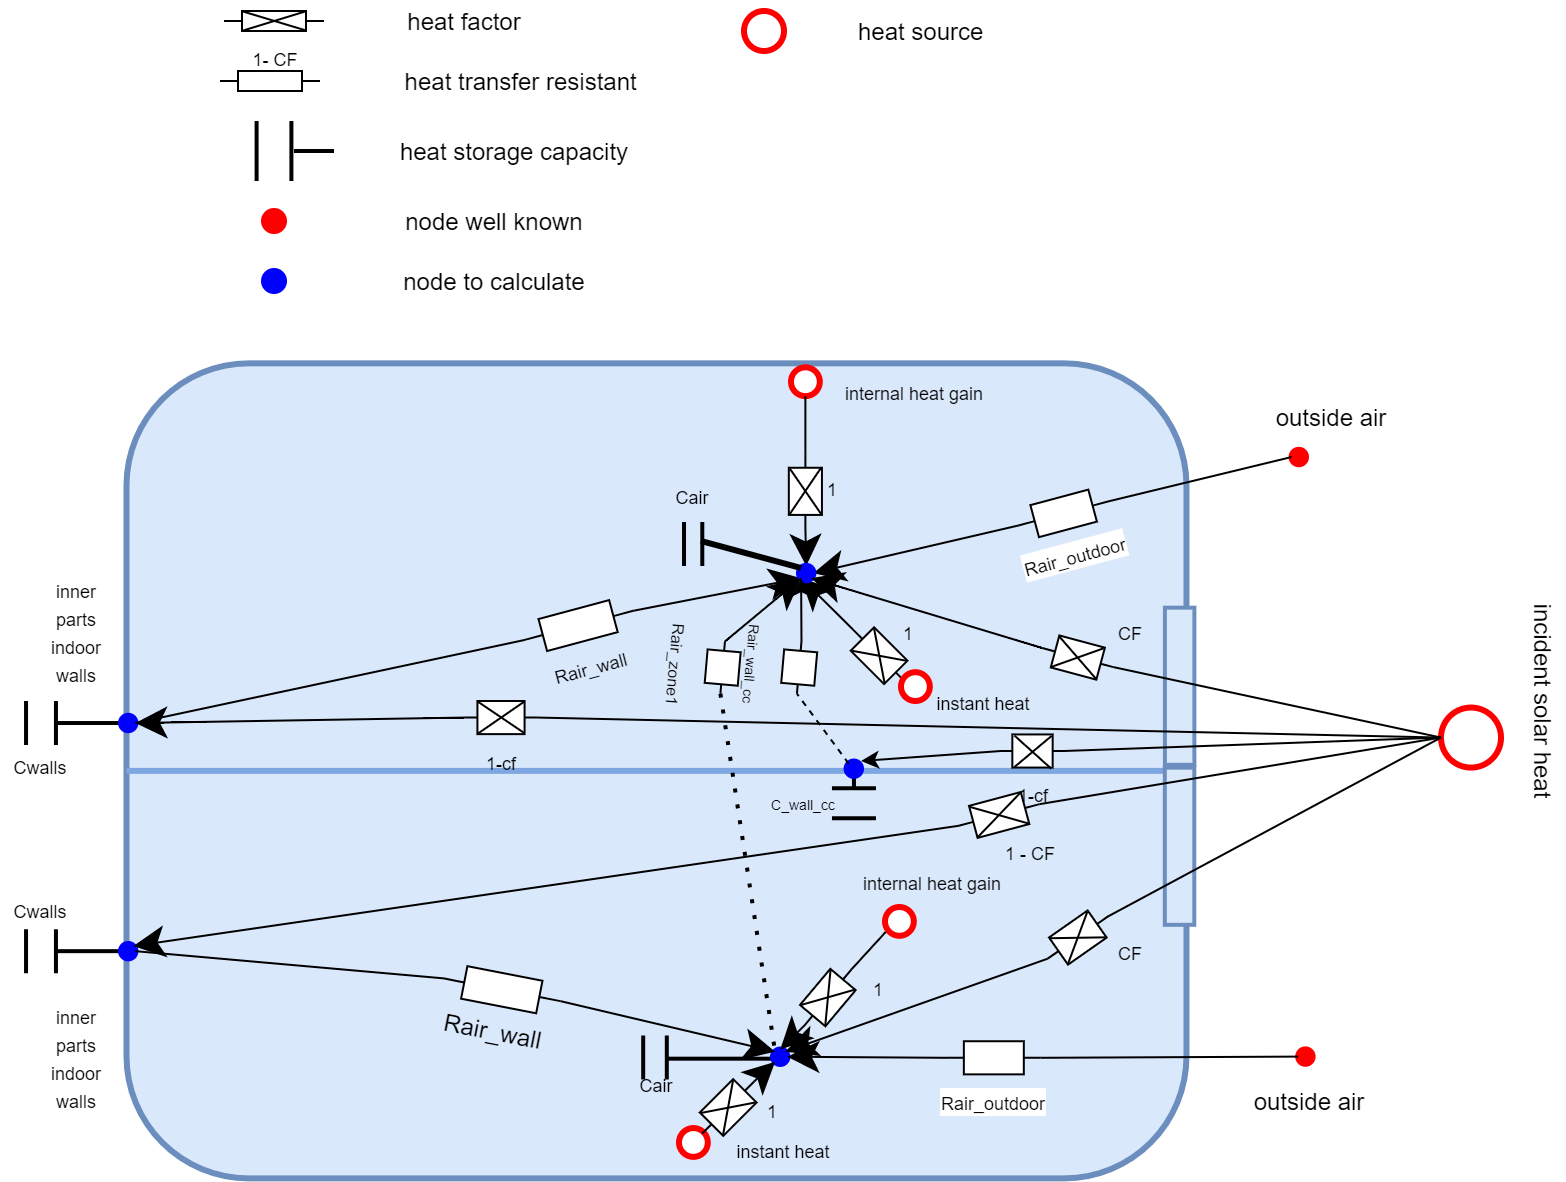
\includegraphics[width=1.0\columnwidth]{Pictures/House_electrical_circuits overview.png}
	\caption[Short title]{Schematic of a 2 zones house model}
	\label{fig:schema7R4C}
	\end{figure} 
	
The equivalent electrical 7R-4C network with components and topology is given in Fig. \ref{fig:elec7R4C}.

\begin{figure}[H]
	\centering
	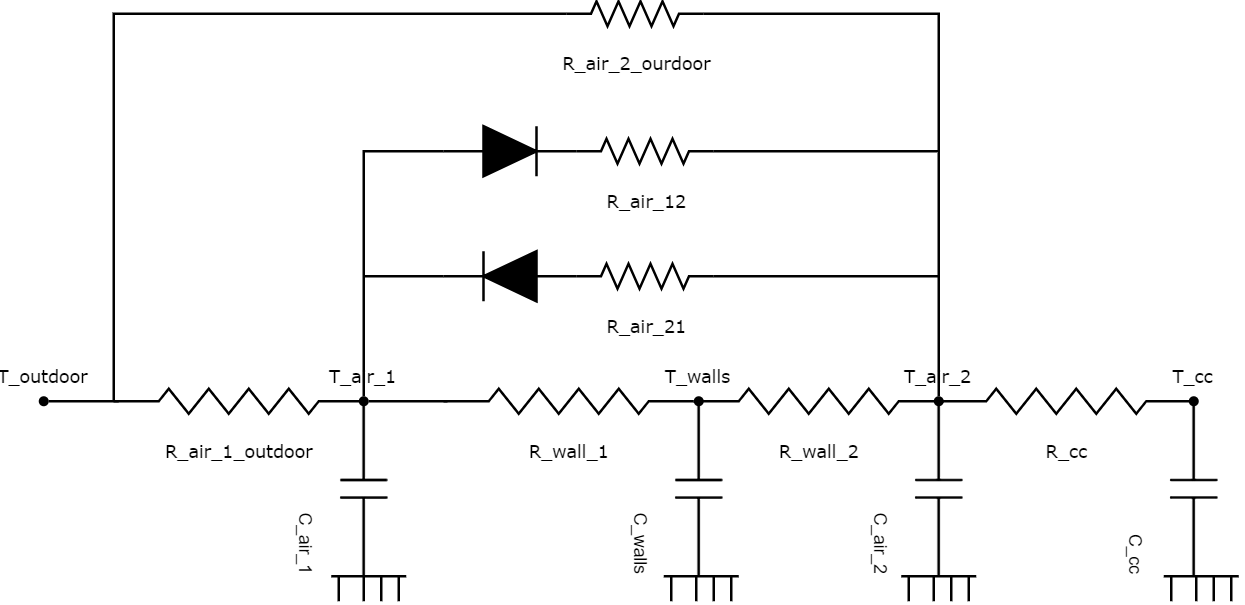
\includegraphics[width=1.0\columnwidth]{Pictures/2_Zones_house_circuits.png}
	\caption[Short title]{R-C circuits of 2 zones house model}
	\label{fig:elec7R4C}
	\end{figure}

with:\\
\begin{itemize}
    \item \texttt{T\_outdoor} : outdoor temperature [$\degr C$] 
    \item \texttt{T\_air\_1}  : zone 1 air temperature [$\degr C$]
    \item \texttt{T\_walls}   : wall temperature [$\degr C$]
    \item \texttt{T\_air\_2}  : zone 2 air temperature [$\degr C$]
    \item \texttt{T\_cc}      : temperature of the concrete layer between zone 1 and zone 2 [$\degr C$]
    \item \texttt{R\_air\_1\_outdoor} : outdoor resistance valus.
    \item \texttt{R\_wall\_1} : walls resistance value.
    \item \texttt{R\_wall\_2} : walls resistance value.
    \item \texttt{R\_cc}      : concrete resistance value.
    \item \texttt{R\_air\_12} : resistance value of air flow from zone 1 to zone 2.
    \item \texttt{R\_air\_21} : resistance value of air flow from zone 2 to zone 1.

\end{itemize}
\newpage
\section{Lumped-element thermal model of a building}

Heat generation and transport inside a building, with heat loss to the surrounding outdoor environment is governed by the same laws of conduction, convection and radiation as elsewhere. A number of approximations is made, however, which will be treated below:

\subsection{Heat Conduction: Fourier's Law}

Heat transport \emph{within} a solid material is governed by conduction, according to Fourier's Law, illustrated in Figure \ref{fig:heatcond_1d}.
One side of a rectangular solid is held at temperature $T_1$, while the opposite side is held at a lower temperature, $T_2$. The other four sides are insulated so that heat can flow only in the $x$-direction. For a given material, it is found that the rate, $\dot{Q_x}$ , at which heat (thermal
energy) is transferred from the hot side to the cold side (the \emph{heat transfer rate}) is proportional to the cross-sectional area, $A$, across which the heat flows; the temperature difference, $T_1 - T_2$; and inversely proportional to
the thickness, $\Delta x$, of the material. That is:

\begin{equation}
	\label{eq:fourierlaw}
	\dot{Q_x} = - kA \frac{\Delta T}{\Delta x}
\end{equation}

\begin{figure}[H]
	\centering
	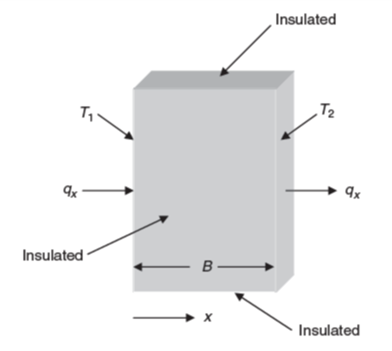
\includegraphics[width=0.5\columnwidth]{Pictures/heat_conduction_1d.png}
	\caption[Short title]{One-dimensional heat conduction in a solid}
	\label{fig:heatcond_1d}
\end{figure} 

The constant of proportionality, $k$, is called the \emph{thermal conductivity}. Equation \eqref{eq:fourierlaw} is also applicable to heat conduction in liquids and gases. However, when temperature differences exist in fluids, convection currents tend to be set up, so that heat is generally not transferred solely by the mechanism of conduction. The thermal conductivity is a property of the material. Values may be found in various handbooks and compendiums of physical property data.

The form of Fourier’s law given by Equation \eqref{eq:fourierlaw} is valid only when the thermal conductivity can be assumed constant. A more general result can be obtained by writing the equation for an element of differential thickness. in the limit as $\Delta x$ approaches zero, $\frac{\Delta T}{\Delta x} \rightarrow \frac{d T}{d x}$. Thus, substituting in Equation \eqref{eq:fourierlaw} gives:

\begin{equation}
	\label{eq:fourierdiff}
	\dot{Q_x} = - kA \frac{d T}{d x}
\end{equation}

Equation \eqref{eq:fourierdiff} is not subject to the restriction of constant $k$. Furthermore, when $k$ is constant, it can be integrated to yield Equation \eqref{eq:fourierlaw}. Hence, Equation \eqref{eq:fourierdiff} is the general one-dimensional form of Fourier’s law. The negative sign is necessary because heat flows in the positive $x$-direction when the temperature decreases in the $x$-direction. Thus, according to the standard sign convention that
$\dot Q_x$ is positive when the heat flow is in the positive $x$-direction, $\dot Q_x$ must be positive when $dT/dx$ is negative. 

\subsubsection{More than one dimension}

It is often convenient to formulate Fourier's Law in the original phrasing: the \emph{heat flux} $ \dot{\varphi}$  is proportional to the \emph{temperature gradient}. We divide \eqref{eq:fourierdiff} by the area to give:

\begin{equation}
	\label{eq:fourierflux}
	\dot{\varphi_x} \equiv \frac{\dot Q_x}{A}- k \frac{d T}{d x}
\end{equation}

where $\dot{\varphi_x}$ is the heat flux. It has units of $\frac{J}{s \cdot m^2} = \frac{W}{m^2}$. 
Thus, the units of $k$ are $\frac{W}{m \cdot K}$.

Equation \eqref{eq:fourierflux} is restricted to the situation in which heat flows in the $x$-direction
only. In the general case in which heat flows in all three coordinate directions, the total heat flux is obtained by vector addition of adding the fluxes in the coordinate directions. Thus,

\begin{equation}
	\label{eq:flux3d}
	\boldsymbol{\dot{\varphi}} = \dot{\varphi_x} \mathbf{i} + \dot{\varphi_y} \mathbf{j} + \dot{\varphi_z} \mathbf{k}
\end{equation}

where $\boldsymbol{\dot{\varphi}}$ is the heat flux vector and \textbf{i}, \textbf{j}, \textbf{k} are unit vectors in the x-, y-, z-directions, respectively.

Each of the component fluxes is given by a one-dimensional Fourier expression as follows:

\begin{equation}
	\begin{aligned}
		\label{eq:fourier3d}
		\dot{\varphi_x} = - k \frac{\partial T}{\partial x} & \qquad & \dot{\varphi_y} = - k \frac{\partial T}{\partial y} & \qquad & \dot{\varphi_z} = - k \frac{\partial T}{\partial z}
	\end{aligned}
\end{equation}

Partial derivatives are used here since the temperature now varies in all three directions. Substituting
the above expressions for the fluxes into Equation \eqref{eq:flux3d} gives:

\begin{equation}
	\label{eq:fouriercart}
	\boldsymbol{\dot{\varphi}} = -k \left(\frac{\partial T}{\partial x} \mathbf{i} + \frac{\partial T}{\partial y} \mathbf{j} + \frac{\partial T}{\partial z} \mathbf{k} \right)
\end{equation}

The vector in parenthesis is the temperature gradient vector, and is denoted by $\nabla T$. Hence,

\begin{equation}
	\label{eq:fouriernabla}
	\boldsymbol{\dot{\varphi}} = -k \nabla T
\end{equation}

Equation \eqref{eq:fouriernabla} is the three-dimensional form of Fourier’s law. It is valid for homogeneous, isotropic materials for which the thermal conductivity is the same in all directions. Fourier’s law states that heat flows in the direction of greatest temperature decrease.

\subsubsection{The Heat Conduction Equation}

The solution of problems involving heat conduction in solids can, in principle, be reduced to the
solution of a single differential equation, the \emph{heat conduction equation}. The equation can be derived
by making a thermal power balance on a differential volume element in the solid. For the case of
conduction in the $x$-direction only, such a volume element is illustrated in Figure \ref{fig:element_1d}. 

\begin{figure}[H]
	\centering
	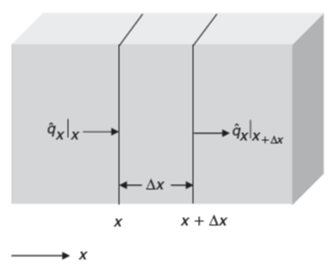
\includegraphics[width=0.5\columnwidth]{Pictures/Element.png}
	\caption[Short title]{Differential element for 1D heat conduction}
	\label{fig:element_1d}
\end{figure}

The rate at which thermal energy enters the volume element across the face at $x$ is given by the
product of the heat flux and the cross-sectional area, $\dot{\varphi_x}|_x \cdot A$.
Similarly, the rate at which thermal energy leaves the element across the face at $x + \Delta x$ is $\dot{\varphi_x}|_{x + \Delta x} \cdot A$. 

A heat generation term appears in the equation because the balance is made on thermal energy, not
total energy. For example, thermal energy may be generated within a solid by an electric current
or by decay of a radioactive material.

For a homogeneous heat source of strength $\dot{q}$ \emph{per unit volume}, the net rate of generation is $\dot{q}A \Delta x$. Finally, the rate of accumulation of heat in the material is given by the time derivative of the thermal energy content of the volume element, which is $\rho c(T - T_{ref} )A\Delta x$, where $T_{ref}$ is an arbitrary reference temperature. Thus, the balance equation
becomes:

\begin{equation}
	\label{eq;heatbalance}
	\left( \dot{\varphi_x}|_x - \dot{\varphi_x}|_{x + \Delta x} \right)A + \dot{q}A \Delta x = \rho c  \frac{\partial T}{\partial t}A\Delta x
\end{equation}

It has been assumed here that the density, $\rho$, and heat capacity, $c$, are constant. 

Dividing by $A \Delta x$ and taking the limit as $\Delta x \rightarrow 0 $ yields:

\begin{equation}
	\rho c  \frac{\partial T}{\partial t} = -\frac{\partial \dot{\varphi_x}}{\partial x} + \dot{q}
\end{equation}

Using Fourier’s law as given by Equation \eqref{eq:fourierflux}, the balance equation becomes:

\begin{equation}
	\rho c  \frac{\partial T}{\partial t} = \frac{\partial}{\partial x} \left(\frac{k \partial T}{\partial x} \right)+ \dot{q}
\end{equation}

When conduction occurs in all three coordinate directions, the balance equation contains y- and
z-derivatives analogous to the x-derivative. The balance equation then becomes:

\begin{equation}
	\label{eq:heat3d}
	\rho c  \frac{\partial T}{\partial x} = \frac{\partial}{\partial x} \left(\frac{k \partial T}{\partial x} \right)  + \frac{\partial}{\partial y} \left(\frac{k \partial T}{\partial y} \right) + \frac{\partial}{\partial z} \left(\frac{k \partial T}{\partial z} \right) + \dot{q}
\end{equation}

When $k$ is constant, it can be taken outside the derivatives and Equation \eqref{eq:heat3d} can be written as:	

\begin{equation}
	\frac{\rho c}{k}  \frac{\partial T}{\partial t} = \frac{\partial^2 T}{\partial x^2}  + \frac{\partial^2 T}{\partial y^2} + \frac{\partial^2 T}{\partial z^2} + \frac{\dot{q}}{k}
\end{equation}

or

\begin{equation}
	\frac{1}{\alpha} \frac{\partial T}{\partial t} = \nabla^2 T + \frac{\dot{q}}{k}
\end{equation}

where $\alpha \equiv k /\rho c$ is the \emph{thermal diffusivity} and $\nabla^2$ is the Laplacian operator. The thermal diffusivity has units of $m^2/s$.


\subsection{Convection: Newton's Law of cooling}

When a solid is \emph{immersed} in a fluid or atmospheric gas, heat transfer on the interface occurs by convection. This phenomenon is governed by Newton's Law of cooling:

“The rate of heat lost by a body is directly proportional to the temperature difference of a body and its surroundings”

\begin{equation}
	\label{eq:newtonlaw}
	\dot{Q_x} = - hA \Delta T
\end{equation}

\subsection{Radiation}

\subsection{Approximations: A Simplified Model}

In building physics, it is often assumed that Fourier's Law is valid in the form of Eq. \eqref{eq:fourierlaw}. This can be done under the condition that 

\begin{equation}
	\begin{aligned}
	    \nabla^2 T \equiv 0 & \rightarrow & \frac{\partial T}{\partial \mathbf{r}} = constant
    \end{aligned}
\end{equation}

\subsection{Lumped-element matrix representation}

We take the 2R-2C lumped-element model from Section 2:

\begin{figure}[H]
	\centering
	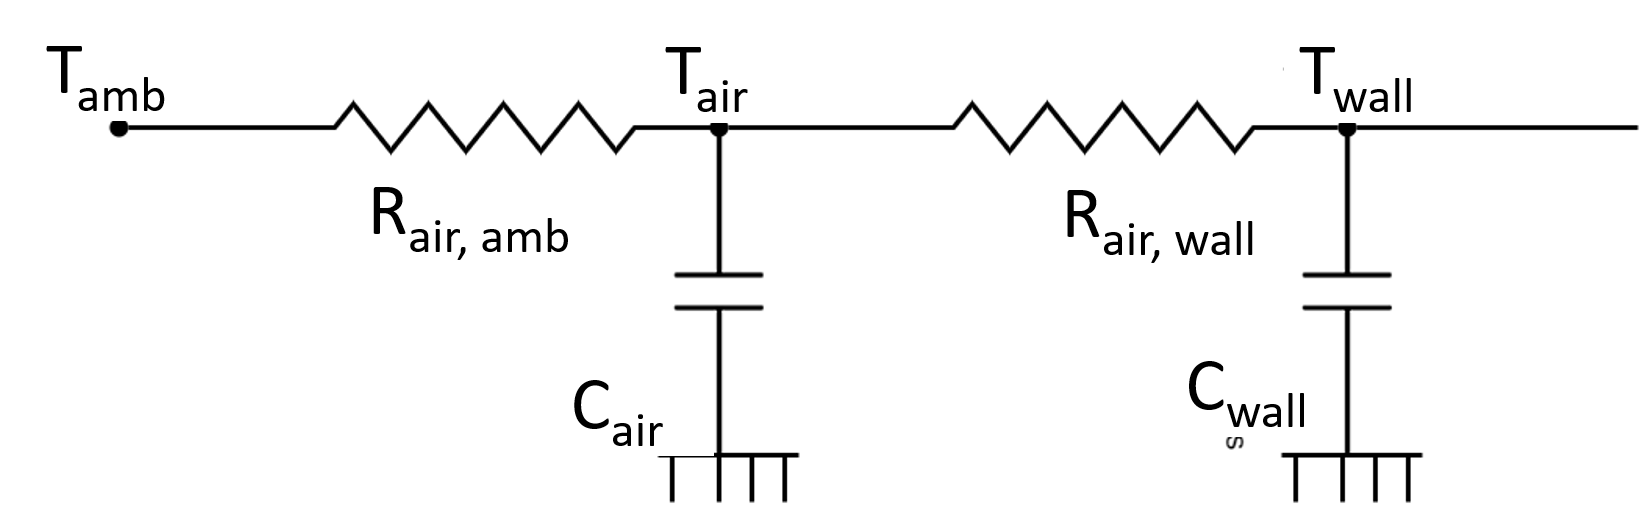
\includegraphics[width=0.7\columnwidth]{Pictures/2R2Cmodel_rev.png}
	\caption[Short title]{2R-2C house model revisited}
	\label{fig:elec2R2Cbis}
\end{figure}

The differential equations are:

\begin{equation}
	\begin{aligned}
	C_{air}\frac{dT_{air}}{dt} &=\frac{T_{amb}-T_{air}}{R_{air, amb}} + \frac{T_{wall}-T_{air}}{R_{air, wall}} + \dot{Q}_{heat, air} + \dot{Q}_{int, air} + \dot{Q}_{solar, air} 
	\\ \\
	C_{wall}\frac{dT_{wall}}{dt} &=\frac{T_{air}-T_{wall}}{R_{air, wall}} + \dot{Q}_{solar, wall}
    \end{aligned}
\end{equation}

Writing out the differential equations in the classical notation:

\begin{equation}
	\begin{aligned}
		C_{air}\frac{dT_{air}}{dt} &= \left[ \frac{-1}{R_{air, amb}} + \frac{-1}{R_{air, wall}} \right]  \cdot T_{air}  + \frac{1}{R_{air, wall}} \cdot T_{wall} + \frac{1}{R_{air, amb}} \cdot T_{amb} + \dot{Q}_{heat, air} + \dot{Q}_{int, air} + \dot{Q}_{solar, air} 
		\\ \\
		C_{wall}\frac{dT_{wall}}{dt} &= \frac{1}{R_{air, wall}} \cdot T_{air} + \frac{-1}{R_{air, wall}}   \cdot T_{wall} + \dot{Q}_{solar, wall}
	\end{aligned}
\end{equation}

The differential equations can be written in matrix notation as:

\begin{subequations}
	\label{eq:matnot}
	\begin{align}
	\mathbf{C} \cdot \boldsymbol{\dot{\theta}} = - \mathbf{K} \cdot \boldsymbol{\theta} + \mathbf{\dot{q}} \\ 
	\mathbf{C} \cdot \boldsymbol{\dot{\theta}} + \mathbf{K} \cdot \boldsymbol{\theta} = \mathbf{\dot{q}}
	\end{align}
\end{subequations}

with:

\begin{equation}
	\mathbf{C} \cdot \boldsymbol{\dot{\theta}} =
	\begin{bmatrix}
		C_{air} & 0 \\
		0 &  C_{wall}
	\end{bmatrix}
    \cdot
    \begin{bmatrix}
    	\frac{dT_{air}}{dt} \\
    	\frac{dT_{wall}}{dt}
    \end{bmatrix}
\end{equation}

\begin{equation}
	\mathbf{K} \cdot \boldsymbol{\theta} =
	\begin{bmatrix}
		\frac{1}{R_{air, amb}} + \frac{1}{R_{air, wall}} & \frac{-1}{R_{air, wall}} \\
		\frac{-1}{R_{air, wall}} &  \frac{1}{R_{air, wall}}
	\end{bmatrix}
	\cdot
	\begin{bmatrix}
		T_{air} \\
		T_{wall}
	\end{bmatrix}
\end{equation}

\begin{equation}
	\mathbf{\dot{q}} =
	\begin{bmatrix}
		\frac{1}{R_{air, amb}} \cdot T_{amb} + \dot{Q}_{heat, air} + \dot{Q}_{int, air} + \dot{Q}_{solar, air} \\
		\dot{Q}_{solar, wall}
	\end{bmatrix}
\end{equation}

Written out, the differential equation according to \eqref{eq:matnot} becomes:

\begin{equation}
	\begin{aligned}
		\begin{bmatrix}
			C_{air} & 0 \\
			0 &  C_{wall}
		\end{bmatrix}
		\cdot
		\begin{bmatrix}
			\frac{dT_{air}}{dt} \\
			\frac{dT_{wall}}{dt}
		\end{bmatrix}
		=
		\begin{bmatrix}
			\frac{-1}{R_{air, amb}} + \frac{-1}{R_{air, wall}} & \frac{1}{R_{air, wall}} \\
			\frac{1}{R_{air, wall}} &  \frac{-1}{R_{air, wall}}
		\end{bmatrix}
		\cdot
		\begin{bmatrix}
			T_{air} \\
			T_{wall}
		\end{bmatrix}
		+ \\ \\
		\begin{bmatrix}
			\frac{1}{R_{air, amb}} \cdot T_{amb} + \dot{Q}_{heat, air} + \dot{Q}_{int, air} + \dot{Q}_{solar, air} \\
			\dot{Q}_{solar, wall}
		\end{bmatrix}
	\end{aligned}
\end{equation}

In the alternative notation:

\begin{equation}
	\begin{aligned}
	\begin{bmatrix}
	    C_{air} & 0 \\
	    0 &  C_{wall}
    \end{bmatrix}
    \cdot
    \begin{bmatrix}
    	\frac{dT_{air}}{dt} \\
    	\frac{dT_{wall}}{dt}
    \end{bmatrix}
    +
    	\begin{bmatrix}
    	\frac{1}{R_{air, amb}} + \frac{1}{R_{air, wall}} & \frac{-1}{R_{air, wall}} \\
    	\frac{-1}{R_{air, wall}} &  \frac{1}{R_{air, wall}}
    \end{bmatrix}
    \cdot
    \begin{bmatrix}
    	T_{air} \\
    	T_{wall}
    \end{bmatrix}
    = \\ \\
    \begin{bmatrix}
        \frac{1}{R_{air, amb}} \cdot T_{amb} + \dot{Q}_{heat, air} + \dot{Q}_{int, air} + \dot{Q}_{solar, air} \\
    	\dot{Q}_{solar, wall}
    \end{bmatrix}
	\end{aligned}
\end{equation}

The lumped-element equations above are systems of \emph{first-order ordinary differential equations} (ODE). The first order derivative is with respect to \emph{time}. The (silent) assumption that heat conduction within the air and the wall of the previous 2R-2C model is \emph{faster} than the exchange of heat at the \emph{interfaces} between air and wall and air and ambient surroundings has replaced all spatial information from the \emph{second-order partial differential equations} (PDE) that govern conductive heat transport \emph{within} materials.

Therefore, the lumped-element equations can be solved by:
\begin{itemize}
	\item the \textsf{odexxx} in Matlab., preferrably \textsf{ode45}.
	\item the \textsf{state-space} module in Simulink, after conversion to a state-space representation.
	\item the \textsf{scipy.integrate.solve\_ivp} function in Python. In older code, \textsf{scipy.integrate.odeint} is still encountered.
	\item in C++ several options exist, similar to the options in Python.
\end{itemize}

The routines in Matlab, Simulink and Python need a \emph{model function} that provides the vector $\boldsymbol{\dot{\theta}}$ for evaluation at any time instance chosen by the algorithm. The equations \eqref{eq:matnot} then should be cast in the following form by left multiplication with $\mathbf{C^{-1}}$.

\begin{subequations}
	\label{eq:matnot_ivp}
	\begin{align}
		\mathbf{C}^{-1} \cdot \mathbf{C} \cdot \boldsymbol{\dot{\theta}} = - \mathbf{C}^{-1} \cdot \mathbf{K} \cdot \boldsymbol{\theta} + \mathbf{C}^{-1} \cdot \mathbf{\dot{q}} \\ 
        \boldsymbol{\dot{\theta}} = - \mathbf{C}^{-1} \cdot \mathbf{K} \cdot \boldsymbol{\theta} + \mathbf{C}^{-1} \cdot \mathbf{\dot{q}}
	\end{align}
\end{subequations}

Since $\mathbf{C}$ is a \emph{diagonal} matrix with positive elements only, its inverse exists and contains the reciprocal elements on its diagonal:

\begin{equation}
	\mathbf{C^{-1}} =
	\begin{bmatrix}
		\frac{1}{C_{air}} & 0 \\
		0 &  \frac{1}{C_{wall}}
	\end{bmatrix}
\end{equation}

This provides the division by the lumped thermal capacitances of the air and wall compartments in the model, necessary for the calculating the derivative vector $\boldsymbol{\dot{\theta}}$ in the model functions. 

\subsection{Extension of the method to larger lumped-element networks}

Take a house model with two stories. Each level in the building is described with a 2R-2C model. Heat transfer occurs between the ground floor and the 1st floor.

\begin{figure}[H]
	\centering
	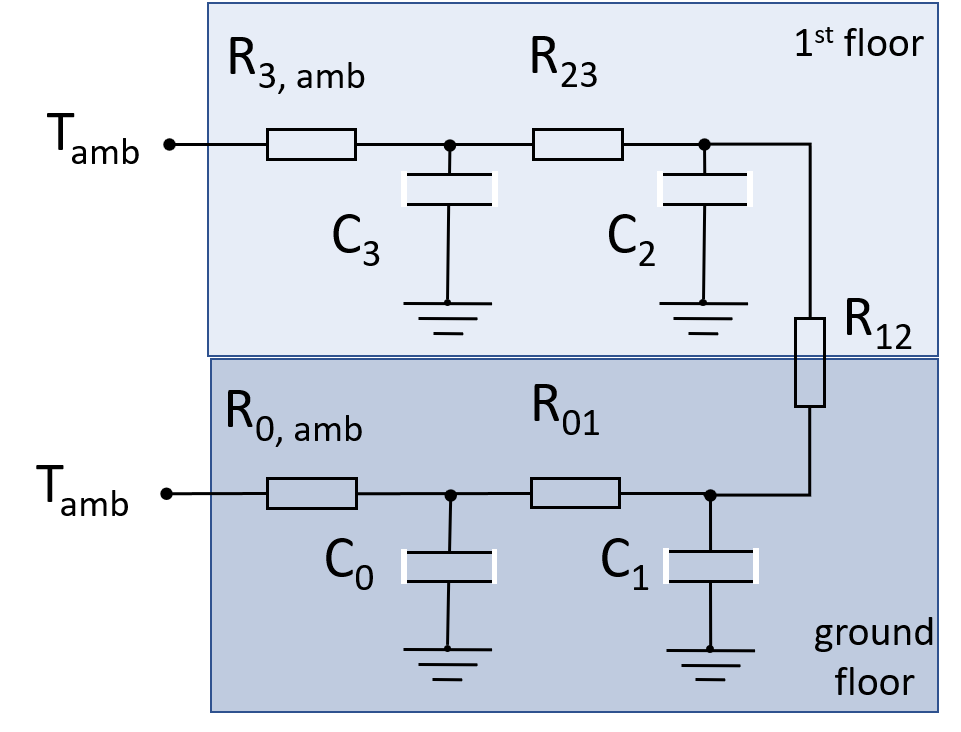
\includegraphics[width=0.6\columnwidth]{Pictures/5R4C.png}
	\caption[Short title]{5R-4C house model}
	\label{fig:elec4R5C}
\end{figure}

\begin{equation}
	\mathbf{C} \cdot \boldsymbol{\dot{\theta}} =
	\begin{bmatrix}
		C_{0} & 0 & 0 & 0\\
		0 &  C_{1} & 0 & 0 \\
		0 & 0 & C_{2} & 0\\
		0 & 0 & 0 & C_{3}
	\end{bmatrix}
	\cdot
	\begin{bmatrix}
		\frac{dT_{0}}{dt} \\
		\frac{dT_{1}}{dt} \\
	    \frac{dT_{2}}{dt} \\
	    \frac{dT_{3}}{dt} 
	\end{bmatrix}
\end{equation}

\begin{equation}
	\mathbf{K} \cdot \boldsymbol{\theta} =
	\begin{bmatrix}
		\frac{1}{R_{0, amb}} + \frac{1}{R_{01}} & \frac{-1}{R_{01}} & 0 & 0 \\
		\frac{-1}{R_{01}} &  \frac{1}{R_{01}} + \frac{1}{R_{12}} & \frac{-1}{R_{12}} & 0 \\
		 0 & \frac{-1}{R_{12}} & \frac{1}{R_{12}} + \frac{1}{R_{23}}  & \frac{-1}{R_{23}}\\
	 	 0 & 0 & \frac{-1}{R_{23}} &  \frac{1}{R_{3, amb}} + \frac{1}{R_{23}} \\
	\end{bmatrix}
	\cdot
	\begin{bmatrix}
		T_{0} \\
		T_{1} \\
		T_{2} \\
		T_{3}
	\end{bmatrix}
\end{equation}

\begin{equation}
	\mathbf{\dot{q}} =
	\begin{bmatrix}
		\frac{1}{R_{0, amb}} \cdot T_{amb} + \dot{Q}_{heat, 0} + \dot{Q}_{int, 0} + \dot{Q}_{solar, 0} \\
		\dot{Q}_{solar, 1} \\
		\dot{Q}_{solar, 2} \\
		\frac{1}{R_{3, amb}} \cdot T_{amb} + \dot{Q}_{heat, 3} + \dot{Q}_{int, 3} + \dot{Q}_{solar, 3}
	\end{bmatrix}
\end{equation}

\subsection{Alternative representation of 5R-4C model}

The 5R4C model of the previous section can be built from two 2R2C models, one for the ground floor and one for the first floor. The thermal resistance between the construction nodes of the ground and first floor is then added, $R_{13}$ in the figure:
 
\begin{figure}[H]
	\centering
	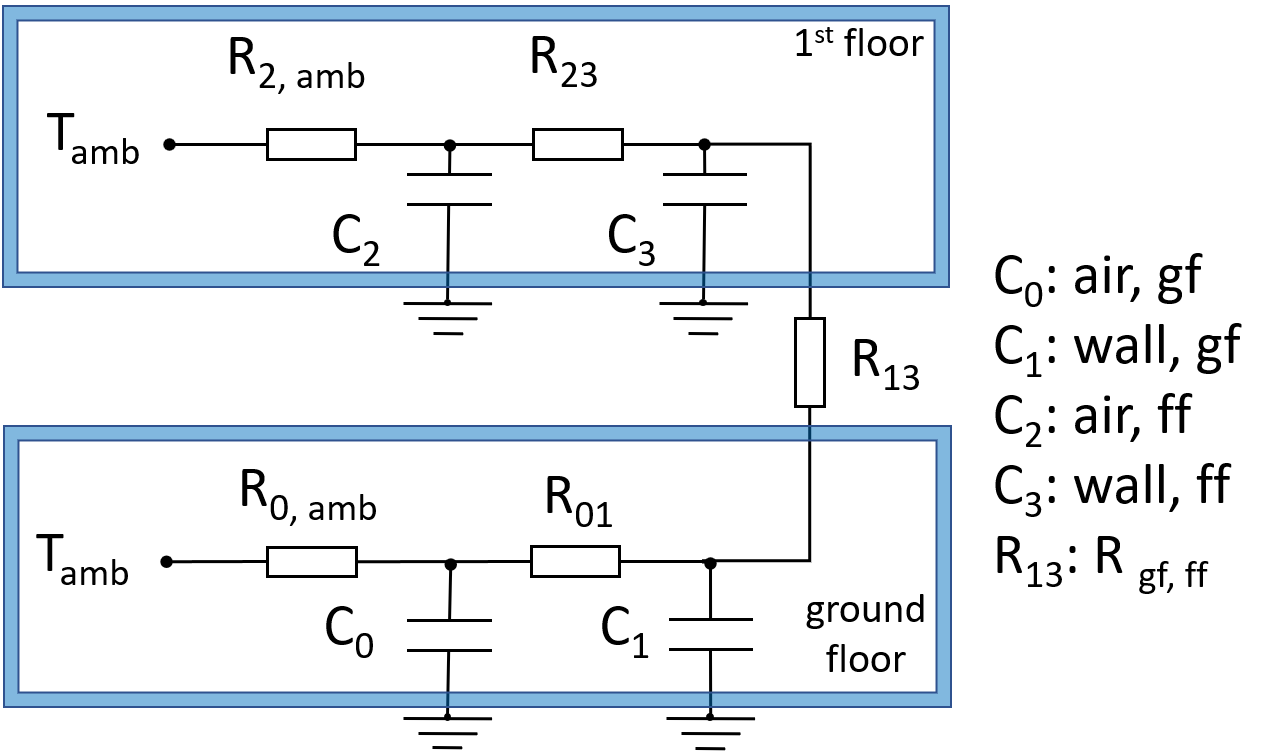
\includegraphics[width=0.6\columnwidth]{Pictures/5R4C_alternative.png}
	\caption[Short title]{5R-4C house model, alternative representation}
	\label{fig:alt5R4C}
\end{figure}

As can be seen in the matrices below, adding $R_{13}$ to the ground floor and first floor "chains" results in a non-symmetric matrix. It has to determined if this disadvantage outweighs the benefit of adding "chains".

\begin{equation}
	\mathbf{C} \cdot \boldsymbol{\dot{\theta}} =
	\begin{bmatrix}
		C_{0} & 0 & 0 & 0\\
		0 &  C_{1} & 0 & 0 \\
		0 & 0 & C_{2} & 0\\
		0 & 0 & 0 & C_{3}
	\end{bmatrix}
	\cdot
	\begin{bmatrix}
		\frac{dT_{0}}{dt} \\
		\frac{dT_{1}}{dt} \\
		\frac{dT_{2}}{dt} \\
		\frac{dT_{3}}{dt} 
	\end{bmatrix}
\end{equation}

\begin{equation}
	\mathbf{K} \cdot \boldsymbol{\theta} =
	\begin{bmatrix}
		\frac{1}{R_{0, amb}} + \frac{1}{R_{01}} & \frac{-1}{R_{01}} & 0 & 0 \\
		\frac{-1}{R_{01}} &  \frac{1}{R_{01}} + \color{red} \frac{1}{R_{13}} & 0 & \color{red} \frac{-1}{R_{13}} \\
		0 & 0 & \frac{1}{R_{2, amb}} + \frac{1}{R_{23}} & \frac{-1}{R_{23}} \\
		0 & \color{red}\frac{-1}{R_{13}} & \frac{-1}{R_{23}}  & \frac{1}{R_{23}} + \color{red}\frac{1}{R_{13}}
	\end{bmatrix}
	\cdot
	\begin{bmatrix}
		T_{0} \\
		T_{1} \\
		T_{2} \\
		T_{3}
	\end{bmatrix}
\end{equation}

\begin{equation}
	\mathbf{\dot{q}} =
	\begin{bmatrix}
		\frac{1}{R_{0, amb}} \cdot T_{amb} + \dot{Q}_{heat, 0} + \dot{Q}_{int, 0} + \dot{Q}_{solar, 0} \\
		\dot{Q}_{solar, 1} \\
		\frac{1}{R_{2, amb}} \cdot T_{amb} + \dot{Q}_{heat, 2} + \dot{Q}_{int, 2} + \dot{Q}_{solar, 2} \\
		\dot{Q}_{solar, 3} 
	\end{bmatrix}
\end{equation}

Renumbering restores the matrices to a symmetric representation:

\begin{figure}[H]
	\centering
	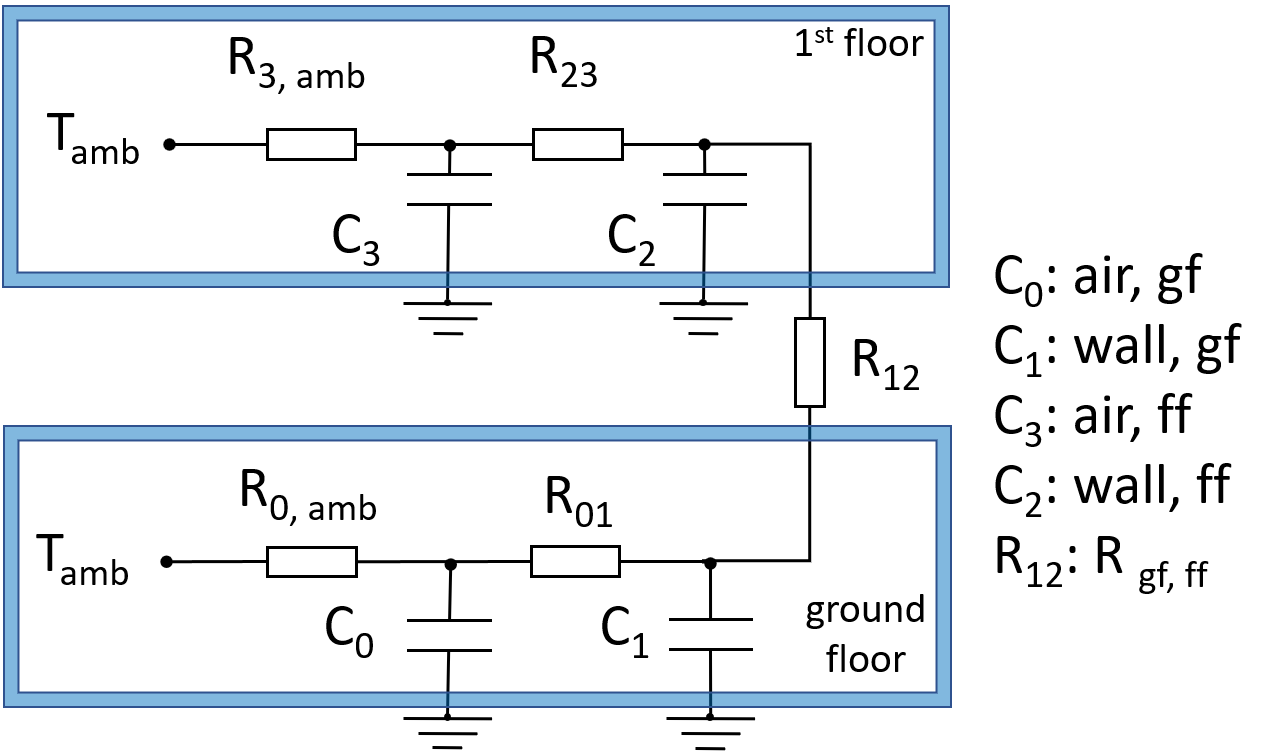
\includegraphics[width=0.6\columnwidth]{Pictures/5R4C_renumbered.png}
	\caption[Short title]{5R-4C house model, alternative representation, renumbered}
	\label{fig:renum5R4C}
\end{figure}

\begin{equation}
	\mathbf{C} \cdot \boldsymbol{\dot{\theta}} =
	\begin{bmatrix}
		C_{0} & 0 & 0 & 0\\
		0 &  C_{1} & 0 & 0 \\
		0 & 0 & C_{2} & 0\\
		0 & 0 & 0 & C_{3}
	\end{bmatrix}
	\cdot
	\begin{bmatrix}
		\frac{dT_{0}}{dt} \\
		\frac{dT_{1}}{dt} \\
		\frac{dT_{2}}{dt} \\
		\frac{dT_{3}}{dt} 
	\end{bmatrix}
\end{equation}

\begin{equation}
	\mathbf{K} \cdot \boldsymbol{\theta} =
	\begin{bmatrix}
		\frac{1}{R_{0, amb}} + \frac{1}{R_{01}} & \frac{-1}{R_{01}} & 0 & 0 \\
		\frac{-1}{R_{01}} &  \frac{1}{R_{01}} + \color{red}\frac{1}{R_{12}} & \color{red}\frac{-1}{R_{12}} & 0 \\
		0 & \color{red} \frac{-1}{R_{12}} & \frac{1}{R_{23}} + \color{red}\frac{1}{R_{12}}   & \frac{-1}{R_{23}}\\
		0 & 0 & \frac{-1}{R_{23}} &  \frac{1}{R_{3, amb}} + \frac{1}{R_{23}} \\
	\end{bmatrix}
	\cdot
	\begin{bmatrix}
		T_{0} \\
		T_{1} \\
		T_{2} \\
		T_{3}
	\end{bmatrix}
\end{equation}

\begin{equation}
	\mathbf{\dot{q}} =
	\begin{bmatrix}
		\frac{1}{R_{0, amb}} \cdot T_{amb} + \dot{Q}_{heat, 0} + \dot{Q}_{int, 0} + \dot{Q}_{solar, 0} \\
		\dot{Q}_{solar, 1} \\
		\dot{Q}_{solar, 2} \\
		\frac{1}{R_{3, amb}} \cdot T_{amb} + \dot{Q}_{heat, 3} + \dot{Q}_{int, 3} + \dot{Q}_{solar, 3}
	\end{bmatrix}
\end{equation}
		
\subsection{2R-2C model with buffervessel}

The "air" and "wall" nodes of the 2R2C model can be extended with "radiator" node. The radiator has a finite heat capacity of itself. Instead of a thermal resistance, the radiator heat exchange in $W/K$ is entered in the model. The radiator emits heat to the "air" node only. In its turn, the radiator is fed from a "buffervessel" node. The buffervessel loses heat to the radiator and is heated up by a gas boiler or alternatively a heat pump. The gas boiler does not heat the house directly, as was the case in the simplest model. A schematic view is given in Fig. \ref{fig:elecbuffer}.

\begin{figure}[H]
	\centering
	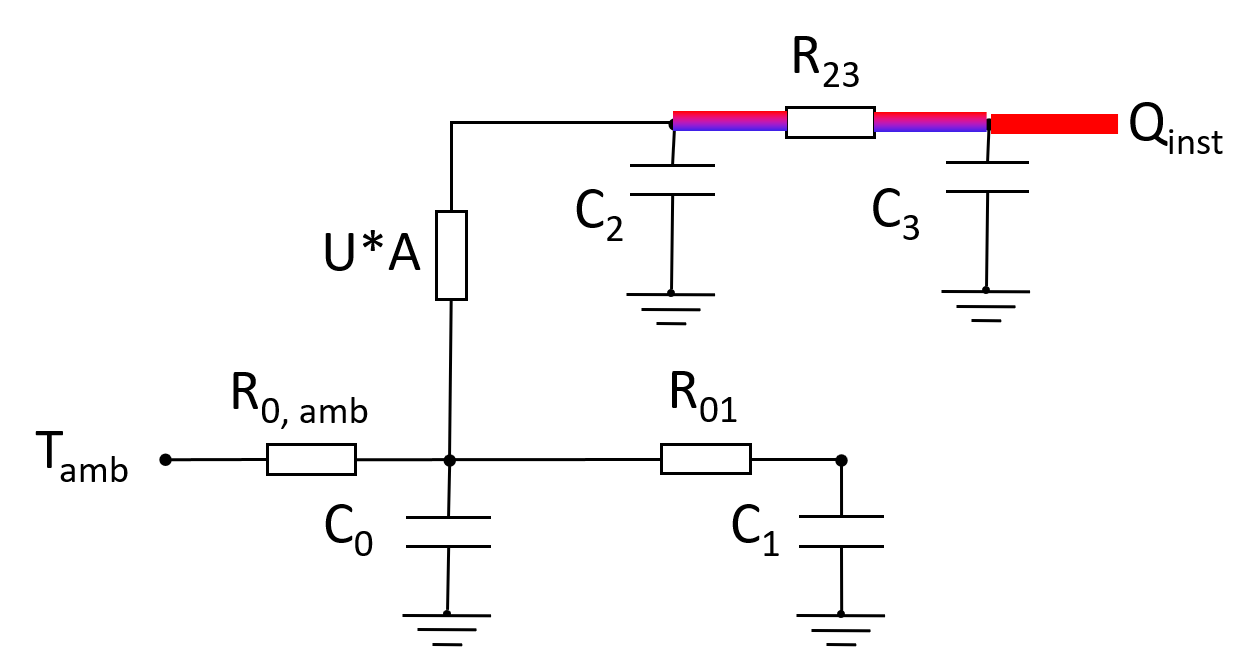
\includegraphics[width=0.7\columnwidth]{Pictures/buffervessel.png}
	\caption[Short title]{2R-2C house model with radiator and buffer vessel}
	\label{fig:buffervessel}
\end{figure} 

The differential equations for heat transport in the model of Fig. \ref{fig:elecbuffer} are:

\begin{equation}
	\begin{aligned}
	    C_{air} \frac{dT_{air}}{dt} &= \frac{T_{outdoor}-T_{air}}{R_{air_{\_}outdoor}} + \frac{T_{wall}-T_{air}}{R_{air_{\_}wall}} + U_{rad} \cdot A_{rad} \cdot (T_{return} - T_{air}) + \dot{Q}_{internal} + \dot{Q}_{solar, 0} \\
	    C_{wall} \frac{dT_{wall}}{dt} &= \frac{T_{air}-T_{wall}}{R_{air_{\_}wall}} + \dot{Q}_{solar, 1} \\
	    C_{rad} \frac{dT_{return}}{dt} &= \dot{m} \cdot c_{p, water} \cdot (T_{buffer} - T_{return}) + U_{rad} \cdot A_{rad} \cdot (T_{air} - T_{return}) \\
		C_{buffer} \frac{dT_{buffer}}{dt} &= \dot{m} \cdot c_{p, water} \cdot ( T_{return} - T_{buffer} ) + \dot{Q}_{inst} \\
	    \frac{dE}{dt} &= \dot{Q}_{inst}
	\end{aligned}
\end{equation}

 A fifth equation, integrating the heat source energy is sometimes added. Re-arranging the terms in the equation gives:
 
\begin{equation}
	\begin{aligned}
		C_{air} \frac{dT_{air}}{dt} &= \left[ \frac{-1}{R_{air_{\_}outdoor}} + \frac{-1}{R_{air_{\_}wall}} +  -1 \cdot U_{rad} \cdot A_{rad} \right] \cdot T_{air} + \frac{T_{wall}}{R_{air_{\_}wall}} + U_{rad} \cdot A_{rad} \cdot T_{return} + \\
		 & \frac{T_{outdoor}}{R_{air_{\_}outdoor}}  + \dot{Q}_{internal} + \dot{Q}_{solar, 0} \\
		C_{wall} \frac{dT_{wall}}{dt} &= \frac{1}{R_{air_{\_}wall}} \cdot T_{air} + \frac{-1}{R_{air_{\_}wall}} \cdot T_{wall} + \dot{Q}_{solar, 1} \\
		C_{rad} \frac{dT_{return}}{dt} &=  U_{rad} \cdot A_{rad} \cdot T_{air} + \left[- U_{rad} \cdot A_{rad} -\dot{m} \cdot c_{p, water}\right] \cdot T_{return} + \dot{m} \cdot c_{p, water} \cdot T_{buffer}\\
		C_{buffer} \frac{dT_{buffer}}{dt} &= \dot{m} \cdot c_{p, water} \cdot T_{return} - \dot{m} \cdot c_{p, water} \cdot T_{buffer} + \dot{Q}_{heat, 3} \\
		\frac{dE}{dt} &= \dot{Q}_{inst}
	\end{aligned}
\end{equation}
Conversion of the equations to a matrix equation yields:
\begin{equation}
	\mathbf{C} \cdot \boldsymbol{\dot{\theta}} =
	\begin{bmatrix}
		C_{0} & 0 & 0 & 0\\
		0 &  C_{1} & 0 & 0 \\
		0 & 0 & C_{2} & 0\\
		0 & 0 & 0 & C_{3}
	\end{bmatrix}
	\cdot
	\begin{bmatrix}
		\frac{dT_{0}}{dt} \\
		\frac{dT_{1}}{dt} \\
		\frac{dT_{2}}{dt} \\
		\frac{dT_{3}}{dt} 
	\end{bmatrix}
\end{equation}

\begin{equation}
	\mathbf{K} \cdot \boldsymbol{\theta} =
	\begin{bmatrix}
		\frac{1}{R_{0, amb}} + \frac{1}{R_{01}} + U \cdot A & \frac{-1}{R_{01}} & -U \cdot A & 0 \\
		\frac{-1}{R_{01}} &  \frac{1}{R_{01}}  & 0 & 0 \\
		-U \cdot A & 0 & U \cdot A + \frac{1}{R_{23}}  & \frac{-1}{R_{23}}\\
		0 & 0 & \frac{-1}{R_{23}} &  \frac{1}{R_{23}} \\
	\end{bmatrix}
	\cdot
	\begin{bmatrix}
		T_{0} \\
		T_{1} \\
		T_{2} \\
		T_{3}
	\end{bmatrix}
\end{equation}

\begin{equation}
	\mathbf{\dot{q}} =
	\begin{bmatrix}
		\frac{1}{R_{0, amb}} \cdot T_{amb} + \dot{Q}_{int, 0} + \dot{Q}_{solar, 0} \\
		\dot{Q}_{solar, 0} \\
		0 \\
		\dot{Q}_{heat, 3}
	\end{bmatrix}
\end{equation}

\subsection{2R-2C model with radiator only}

\begin{figure}[H]
	\centering
	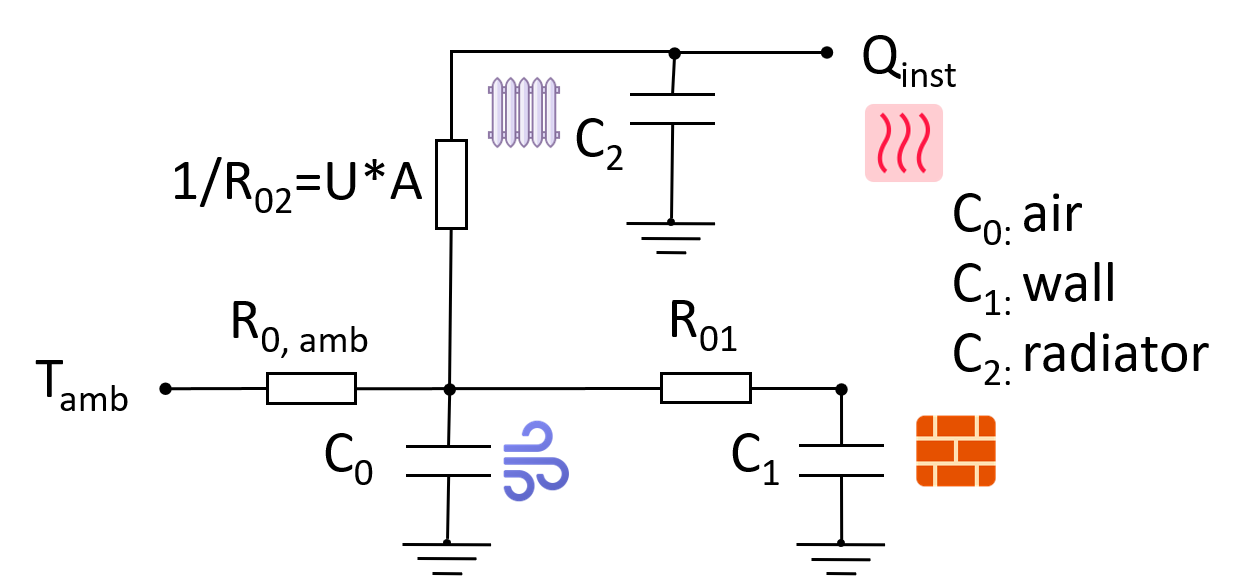
\includegraphics[width=0.7\columnwidth]{Pictures/2R2C_radiator.png}
	\caption[Short title]{2R-2C house model with radiator only}
	\label{fig:2R2Cradiator}
\end{figure} 

The rate of heat transfer from a radiator to the ambient(room) air can be calculated as follows \cite{heatemissionrad}:

\begin{equation}
	\begin{aligned}
	    P & = P_{50} \cdot \left[\Delta T_{LMTD} \cdot \frac{1}{49.32}\right]^n \\
	    \Delta T_{LMTD} & = \frac{ T_{inlet} - T_{return} }{\ln \frac{ T_{inlet} - T_{ambient} }{T_{return} - T_{ambient}}} \\
	    n & = 1.33
    \end{aligned}
\end{equation}

This is sometimes simplified to:

\begin{equation}
	\begin{aligned}
		P & = U \cdot A \cdot \Delta T_{LMTD} \\
		\Delta T_{LMTD} & = \frac{ T_{inlet} - T_{return} }{\ln \frac{ T_{inlet} - T_{ambient} }{T_{return} - T_{ambient}}}
	\end{aligned}
\end{equation}

or simplified to \cite{NEN442, OEM442}:

\begin{equation}
	\begin{aligned}
		P & = K_m \cdot \Delta T^n \\
		\Delta T & = \frac{ T_{inlet} + T_{return} }{2} - {T_{ambient}}
	\end{aligned}
\end{equation}

The differential equations for heat transport in the model of Fig.~\ref{fig:2R2Cradiator} are:

\begin{equation}
	\begin{aligned}
		C_{air} \frac{dT_{air}}{dt} &= \frac{T_{outdoor}-T_{air}}{R_{air_{\_}outdoor}} + \frac{T_{wall}-T_{air}}{R_{air_{\_}wall}} + U_{rad} \cdot A_{rad} \cdot (T_{rad} - T_{air}) + \dot{Q}_{internal} + \dot{Q}_{solar, 0} \\
		C_{wall} \frac{dT_{wall}}{dt} &= \frac{T_{air}-T_{wall}}{R_{air_{\_}wall}} + \dot{Q}_{solar, 1} \\
		C_{rad} \frac{dT_{rad}}{dt} &= \dot{Q}_{inst} + U_{rad} \cdot A_{rad} \cdot (T_{air} - T_{rad}) \\
	\end{aligned}
\end{equation}

Re-arranging the terms in the equation gives:

\begin{equation}
	\begin{aligned}
		C_{air} \frac{dT_{air}}{dt} &= \left[ \frac{-1}{R_{air_{\_}outdoor}} + \frac{-1}{R_{air_{\_}wall}} +  -1 \cdot U_{rad} \cdot A_{rad} \right] \cdot T_{air} + \frac{T_{wall}}{R_{air_{\_}wall}} +  U_{rad} \cdot A_{rad} \cdot T_{rad} + \\
		& \frac{T_{outdoor}}{R_{air_{\_}outdoor}}  + \dot{Q}_{internal} + \dot{Q}_{solar, 0} \\
		C_{wall} \frac{dT_{wall}}{dt} &= \frac{1}{R_{air_{\_}wall}} \cdot T_{air} + \frac{-1}{R_{air_{\_}wall}} \cdot T_{wall} + \dot{Q}_{solar, 1} \\
		C_{rad} \frac{dT_{rad}}{dt} &=  U_{rad} \cdot A_{rad} \cdot T_{air} - U_{rad} \cdot A_{rad} \cdot T_{rad} + \dot{Q}_{heat, 2}\\
	\end{aligned}
\end{equation}
Conversion of the equations to a matrix equation yields:
\begin{equation}
	\mathbf{C} \cdot \boldsymbol{\dot{\theta}} =
	\begin{bmatrix}
		C_{0} & 0 & 0 \\
		0 &  C_{1} & 0  \\
		0 & 0 & C_{2} 
	\end{bmatrix}
	\cdot
	\begin{bmatrix}
		\frac{dT_{0}}{dt} \\
		\frac{dT_{1}}{dt} \\
		\frac{dT_{2}}{dt} 
	\end{bmatrix}
\end{equation}

\begin{equation}
	\mathbf{K} \cdot \boldsymbol{\theta} =
	\begin{bmatrix}
		\frac{1}{R_{0, amb}} + \frac{1}{R_{01}} + U \cdot A & \frac{-1}{R_{01}} & -U \cdot A  \\
		\frac{-1}{R_{01}} &  \frac{1}{R_{01}}  & 0  \\
		-U \cdot A & 0 & U \cdot A 
	\end{bmatrix}
	\cdot
	\begin{bmatrix}
		T_{0} \\
		T_{1} \\
		T_{2}
	\end{bmatrix}
\end{equation}

\begin{equation}
	\mathbf{\dot{q}} =
	\begin{bmatrix}
		\frac{1}{R_{0, amb}} \cdot T_{amb} + \dot{Q}_{int, 0} + \dot{Q}_{solar, 0} \\
		\dot{Q}_{solar, 1} \\
		\dot{Q}_{heat, 2}
	\end{bmatrix}
\end{equation}


\begin{figure}[H]
	\centering
	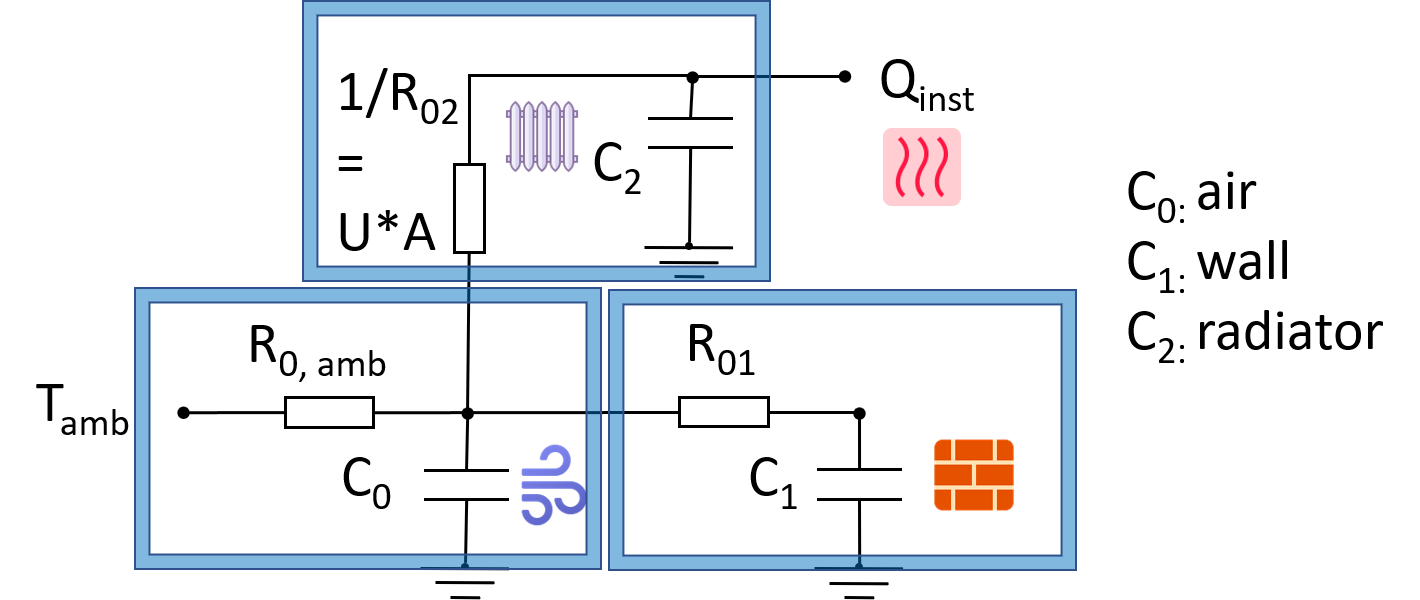
\includegraphics[width=0.7\columnwidth]{Pictures/2R2C_radiator_chains.png}
	\caption[Short title]{2R-2C house model with radiator in 3 chains}
	\label{fig:2R2Cradiator_chains}
\end{figure} 

Starting with the basic 2R2C model we write down the matrices. Note that the heat source for the house is omitted at first. Solar energy entering the house is partitioned between air and wall, Heat generated due to the presence and activities of inhabitants is added to the air node:

\begin{equation}
	\mathbf{C} \cdot \boldsymbol{\dot{\theta}} =
	\begin{bmatrix}
		C_{0} & 0 \\
		0 &  C_{1}
	\end{bmatrix}
	\cdot
	\begin{bmatrix}
		\frac{dT_{0}}{dt} \\
		\frac{dT_{1}}{dt}
	\end{bmatrix}
\end{equation}

\begin{equation}
	\mathbf{K} \cdot \boldsymbol{\theta} =
	\begin{bmatrix}
		\frac{1}{R_{0, amb}} + \frac{1}{R_{01}} & \frac{-1}{R_{01}} \\
		\frac{-1}{R_{01}} &  \frac{1}{R_{01}}
	\end{bmatrix}
	\cdot
	\begin{bmatrix}
		T_{0} \\
		T_{1}
	\end{bmatrix}
\end{equation}

\begin{equation}
	\mathbf{\dot{q}} =
	\begin{bmatrix}
		\frac{1}{R_{0, amb}} \cdot T_{amb} + \dot{Q}_{int, 0} + \dot{Q}_{solar, 0} \\
		\dot{Q}_{solar, 1}
	\end{bmatrix}
\end{equation}

As a third link in the chain, a radiator is added, with a heat capacity $C_{rad}$ and a heat delivery $U \cdot A \cdot (T_{rad} - T_{air})$ to the air node. The heat source $\dot{Q}_{inst}$ is now connected to the radiator.

\begin{equation}
	\mathbf{C} \cdot \boldsymbol{\dot{\theta}} =
	\begin{bmatrix}
		C_{0} & 0 & \color{red} 0 \\
		0 &  C_{1} & \color{red} 0  \\
		\color{red} 0 & \color{red} 0 & \color{red} C_{2} 
	\end{bmatrix}
	\cdot
	\begin{bmatrix}
		\frac{dT_{0}}{dt} \\
		\frac{dT_{1}}{dt} \\
		\color{red}\frac{dT_{2}}{dt} 
	\end{bmatrix}
\end{equation}

\begin{equation}
	\mathbf{K} \cdot \boldsymbol{\theta} =
	\begin{bmatrix}
		\frac{1}{R_{0, amb}} + \frac{1}{R_{01}} {\color{red}+ U \cdot A} & \frac{-1}{R_{01}} & {\color{red}-U \cdot A}  \\
		\frac{-1}{R_{01}} &  \frac{1}{R_{01}}  & \color{red} 0  \\
		{\color{red}-U \cdot A} & \color{red} 0 & {\color{red}U \cdot A }
	\end{bmatrix}
	\cdot
	\begin{bmatrix}
		T_{0} \\
		T_{1} \\
	   \color{red}T_{2}
	\end{bmatrix}
\end{equation}

\begin{equation}
	\mathbf{\dot{q}} =
	\begin{bmatrix}
		\frac{1}{R_{0, amb}} \cdot T_{amb} + \dot{Q}_{int, 0} + \dot{Q}_{solar, 0} \\
		\dot{Q}_{solar, 1} \\
		\color{red} \dot{Q}_{heat, 2}
	\end{bmatrix}
\end{equation}

In this example, it becomes visible (in red) that the rank of the $C$- and $K$-matrix, and the $\dot{q}$-vector is extended by 1. The heat capacity of the radiator is included as an extra \emph{diagonal} element in the $C$-matrix. The heat delivery from the radiator to the indoor air is added to or subtracted from the {00}, {22}, {02} and {20} elements of th $K$-matrix, so that it remains a \emph{symmetric} matrix. The heater is connected to the radiator, represented by element {2} of the $\dot{q}$-vector. 
%\usepackage{xcolor}

\subsection{2R2C revisited: 2R3C}
The 2R2C model as represented in \ref{fig:elec2R2C} treats the node of the outside temperature ($T_{amb}$) differently from the other nodes, $T_{air}$ and $T_{walls}$.  This representation is inconsistent, and actually incomplete. Implicitly, the model links a source/sink to the node that controls the outdoor temperature. In literature, one can find models in which this source has been made explicit, such as in \cite{achterbos}. It seems that this representation has been lost over time. 

In order to complete the analogy with the other nodes in the model we can connect an additional capacitor ($C_amb$). The capacity will be tending to infinity, as we assume the outside temperature not to change due to heat exchange with the house.

\todo{todo:figure including a source and capacitor}

Adding the capacitor and the source also will change the equations. Actually, it results in a more structured set of equations. The equations will be as follows:
\begin{equation}
	\mathbf{C} \cdot \boldsymbol{\dot{\theta}} =
	\begin{bmatrix}
		C_{amb} & 0 & 0\\
		0 &  C_{air} & 0   \\
		0 & 0 & C_{wall} 
	\end{bmatrix}
	\cdot
	\begin{bmatrix}
		\frac{dT_{amb}}{dt} \\
		\frac{dT_{air}}{dt} \\
		\frac{dT_{wall}}{dt} 
	\end{bmatrix}
\end{equation}

\begin{equation}
	\mathbf{K} \cdot \boldsymbol{\theta} =
	\begin{bmatrix}
		\frac{1}{R_{0, amb}}  & \frac{-1}{R_{amb,air}} & 0  \\
		\frac{-1}{R_{amb, air}} &  \frac{1}{R_{01}} + \frac{1}{R_{air,wall}} &  \frac{-1}{R_{air,wall}} \\
		 0 & \frac{-1}{R_{air, wall}}  & \frac{1}{R_{air,wall}} 
	\end{bmatrix}
	\cdot
	\begin{bmatrix}
		T_{amb} \\
		T_{air} \\
		T_{wall}
	\end{bmatrix}
\end{equation}

\begin{equation}
	\mathbf{\dot{q}} =
	\begin{bmatrix}
		\dot{Q}_{amb}\\
		\dot{Q}_{air} \\
		\dot{Q}_{wall} 
	\end{bmatrix}
\end{equation}

In the equations we now see that the matrix $K$ represents the interaction between the different heat capacitors. The structure of $K$ is such that the sum over the rows will always be zero, where the diagonal elements equal the negative sum of the off-diagonal elements. The off-diagonal elements are equal to (minus) conductance factor $\frac{-1}{R}$ between the respective connected nodes. 

The vector $\dot{q}$ contains all heat sources (and sinks). 

Generalizing the idea above, alternative models can be easily constructed using a graph. In the graph each node is labelled with a heat capacity $C_i$, and temperature $T_i$. Nodes $i$ and $j$ can be connected by an edge labelled with $R_{i,j}$, where $\frac{1}{R_{i,j}}$ represents the heat conductance between the two nodes. The $K$-matrix is the connectivity matrix of the graph, where $K_{i,j} = \frac{-1}{R_{i,j}}$. The diagonal elements, $K{i,i}$ are set such that the sums over the rows will be equal to zero.
 

Additionally, each node can be connected to a source or sink. The heat generated or absorbed at each node will be added through the vector $\dot{q}$.

\subsubsection{example: 2R-2C house with buffer}

   


\subsection{Package "housemodel"}

The repository "\textsf{twozone\_housemodel-git}" contains the modules for the house model. The customary way to organize the modules is to make a \emph{Python package} with \emph{subpackages}. This opens up the possibility of publishing the package on PyPi, so that it can be imported.

See: \url{https://pypi.org/}

From commit \textsf{e74ce58} the files in the \textsf{twozone\_housemodel-git} repository are organized as a package. The proposed structure, implemented in this commit, is:

\dirtree{%
	.1 twozone\_housemodel-git.
	.2 housemodel.
	.3 \_\_init\_\_.py.
	.3 controls.
	.4 \_\_init\_\_.py.
	.3 solvers.
	.4 \_\_init\_\_.py.
	.3 sourcesink.
	.4 \_\_init\_\_.py.
	.3 tools.
	.4 \_\_init\_\_.py.
	.2 tests.
	.3 \_\_init\_\_.py.
	.3 context1.py.
	.3 test\_*.py.
} 

\begin{itemize}
	\item the \emph{repository root} \textsf{twozone\_housemodel-git} contains the simulation scripts and configuration files (for now) 
	\item the \emph{package root} \textsf{housemodel} contains the complete package. This can be seen since it contains an (empty) \textsf{\_\_init\_\_.py} module.
	\item the \emph{subpackage} folders contain the modules with common functions and classes for all simulations. They each contain an (empty) \textsf{\_\_init\_\_.py} module.
	\item a \textsf{tests} folder is placed carefully as a subfolder of the \emph{repository root}. 
	See: \url{https://docs.python-guide.org/writing/structure/} for the underlying philosophy. Here, testing modules (scripts) can be placed. If the names of the test scripts start with \textsf{test\_}, they can be automatically run with the \textsf{pytest} Python package.
\end{itemize}

\textit{Note}: Running the simulations and tests is best done from the \emph{repository root}. All simulations and tests have been updated to find the package, subpackages and configuration files from this directory.

\section{Finite-element discretization}

\subsection{Heat pump discretization}

Het algemene model van de warmtepomp en airco wordt afgeleid met behulp van het volgende geschematiseerde black box model:

\subsection{Buffer vessel discretization}

Als voorbeeld van een model met warmtestromen en warmtediffusie wordt het volgende model van
een buffervat beschouwd:

\begin{figure}[H]
	\centering
	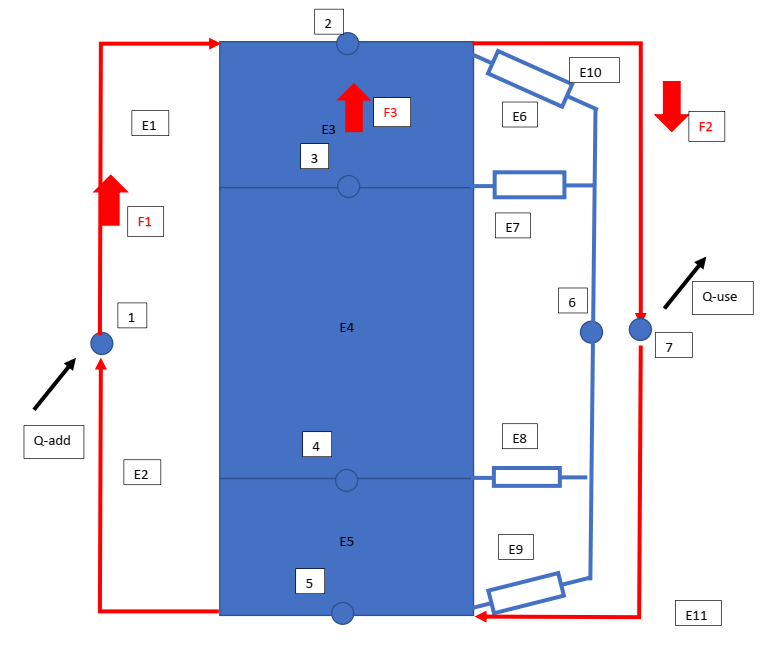
\includegraphics[width=0.7\columnwidth]{Pictures/FEwatervat.png}
	\caption[Short title]{Finite-element buffer vessel}
	\label{fig:FEbuffervessel}
\end{figure}

Dit is een buffervat in een verwarmingsinstallatie.

Voor het modelleren hiervan wordt gebruik gemaakt van een tweetal universele elementen:

\begin{enumerate}
	\item Exchange element. Dit element beschrijft warmtetransportt via een vloeistofstroom $F$ door het element en warmtetransport door geleiding. Het element kan een warmtecapaciteit
	hebben.
	\item Een puntbron. Deze bron beschrijft warmteontwikkeling of warmte-onttrekking in een punt.
\end{enumerate}

Het vat is verdeeld in 3 niveaus over de hoogte:
\begin{enumerate}
	\item Bovenzijde vat (element 3)
	\item Midden vat( element 4 )
	\item Onderzijde vat (element 5 )
\end{enumerate}

In het vat is sprake van:
\begin{itemize}
	\item Warmteverlies naar andere temperatuurniveau ’s en naar de omgeving. De
	omgevingstemperatuur in dit model is gegeven door de temperatuur in punt 7.
	De elementen die het volume van het vat beschrijven (E3,E4 en E5) wisselen warmte uit naar
	elkaar en naar punt 6.
	\item Warmtetransport door waterstromen. In waterstromen buiten het vat wordt warmte
	onttrokken of toegevoegd. In het vat is een waterstroom die zorgt voor het kortsluiten van
	de kringlopen.
\end{itemize}

Deze beide mechanismen worden meegenomen in het model.

Er wordt verondersteld dat gebruik wordt gemaakt van gelaagdheid. Boven in het vat heerst een
hogere temperatuur dan onderin het vat. Daarnaast is er sprake van een tweetal leidingen waarin
warmte wordt uitgewisseld met de omgeving:

\begin{itemize}
	\item Een leiding waarin warmte wordt toegevoegd aan het vat $\dot{Q}_{add}$. Deze leiding neemt
	vloeistof (water) onder uit het vat (punt 5), verhoogt de temperatuur door warmte-inbreng
	(punt 1) en brengt het water boven in het vat weer in. Deze leiding bestaat uit de
	elementen E1 (boven) en E2 (onder). In deze leiding is een vloeistofstroom $F_1 (kJ/(K·s))$
	aanwezig die de warmte transporteert.
	\item Een leiding waarin warmte wordt onttrokken aan het vat $\dot{Q}_{use}$. Deze leiding neemt vloeistof (water) boven uit het vat (punt 2), verlaagt de temperatuur door warmteonttrekking (punt 7) en brengt het water boven in het vat weer in. Deze leiding bestaat uit	de elementen E10 (boven) en E11 (onder). In deze leiding is een vloeistofstroom $F_2 (kJ/(K·s))$ aanwezig die de warmte transporteert.
\end{itemize}

\subsection{Matrixvergelijking}

Voor het oplossen van de temperatuurverdeling wordt per knooppunt een energiebalans opgesteld.
Deze energiebalans resulteert in een matrixvergelijking.

\begin{equation}
	\begin{aligned}
	    \mathbf{K \theta + C \dot{\theta}} = \mathbf{\dot{q}}	    	
	\end{aligned}
\end{equation}

$K$: de warmtegeleidingsmatrix (W/K)
$C$: de warmtecapaciteitsmatrix (J/K)
$\theta$: de temperatuursvector (K)
$\dot{\theta}$: de tijdsafgeleide van de temperatuursvector (K/s)
$\dot{q}$: de vector met thermische brontermen (W)

\subsection{Elementen in de stroming}

Om te komen tot het matrixmodel wordt begonnen met één exchange element zoals hierboven
geïntroduceerd (E1,E2,E3,E4,E5,E10,E11). Dit element bevat 2 knooppunten. De volgende veronderstellingen worden gedaan:

\begin{itemize}
	\item Het element bevat 2 knooppunten waarmee deze verbonden is met de omgeving. De
	nummering bedraagt: $n_1$ en $n_2$.
	\item Binnen het element heerst een lineair verlopende temperatuur, van knooppunt naar
	knooppunt.
	\item Binnen het element is een vloeistofstroom $F$ die zorgt voor additioneel warmtetransport. De stroomrichting is van knooppunt 1 naar knooppunt 2.
	\item De warmtecapaciteit van het element wordt evenredig verdeeld over de knooppunten.
\end{itemize}

De warmtestroom vanuit het element naar knoopunten 1 en 2 moet in balans zijn met de andere
warmtestromen en de warmtegeneratie in de betreffende knooppunten.

\begin{figure}[H]
	\centering
	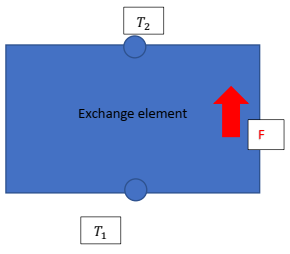
\includegraphics[width=0.7\columnwidth]{Pictures/exchange_element.png}
	\caption[Short title]{Exchange element buffer vessel}
	\label{fig:exchange_element}
\end{figure}

Voor de warmtestromen vanaf knooppunt 1 geldt:

\begin{equation}
	\begin{aligned}
		(T_1 - T_2) \cdot \frac{1}{R_e} + C_{e1,1} \cdot \frac{dT_1}{dT} = \dot{Q}_{ext,1}	    	
	\end{aligned}
\end{equation}

$T_1$: temperatuur in knooppunt 1 \\
$T_2$: temperatuur in knooppunt 2 \\
$R_e$: warmteweerstand voor geleiding tussen knooppunt 1 en 2 \\
$C_{e1,1}$: warmtecapaciteit in knooppunt 1 van element 1 \\
$\frac{dT_1}{dT}$: temperatuursverandering in de tijd in knooppunt 1 \\
$\dot{Q}_{ext,1}$: externe warmtetoevoer in knooppunt 1 \\

De vloeistofstroom $F$ vanuit knooppunt $T_1$ heeft dezelfde temperatuur als $T_1$ en heeft dus geen invloed op de temperatuur in $T_1$.

Voor de warmtestromen vanaf punt 2 geldt:

\begin{equation}
	\begin{aligned}
		(T_2 - T_1) \cdot \frac{1}{R_e} + F \cdot (T_2 - T_1) + C_{e1,2} \cdot \frac{dT_2}{dT} = \dot{Q}_{ext,2}	    	
	\end{aligned}
\end{equation}

$C_{e1,2}$: warmtecapaciteit in knooppunt 2 van element 1 \\
$\frac{dT_2}{dT}$: temperatuursverandering in de tijd in knooppunt 2 \\
$\dot{Q}_{ext,2}$: externe warmtetoevoer in knooppunt 2 \\

In matrixnotatie:

\begin{equation}
	\begin{aligned}
	\begin{bmatrix}
	    1/R_e & -1/R_e \\
	    -1/R_e -F &  1/R_e + F
    \end{bmatrix}
    \cdot
    \begin{bmatrix}
    	T_1 \\
    	T_2
    \end{bmatrix}
    +
    	\begin{bmatrix}
    	C_{e1,1} & 0 \\
    	0 &  C_{e1,2}
    \end{bmatrix}
    \cdot
    \begin{bmatrix}
    	\frac{dT_1}{dt} \\
	    \frac{dT_2}{dt}
    \end{bmatrix}	
    =
        \begin{bmatrix}
    	\dot{Q}_{ext,1} \\
    	\dot{Q}_{ext,2}
    \end{bmatrix}  	
	\end{aligned}
\end{equation}

Merk op dat door de aanwezigheid van een vloeistofstroom $F$, de geleidingsmatrix niet langer symmetrisch is.

Daarnaast wordt gebruik gemaakt van elementen die alleen een warmteweerstand weergeven. Deze
elementen (E6,E7,E8 en E9) kunnen worden gerepresenteerd met de volgende matrixvergelijking

\begin{equation}
	\begin{aligned}
		\begin{bmatrix}
			1/R_e & -1/R_e \\
			-1/R_e &  1/R_e
		\end{bmatrix}
		\cdot
		\begin{bmatrix}
			T_1 \\
			T_2
		\end{bmatrix}	
		=
		\begin{bmatrix}
			\dot{Q}_{ext,1} \\
			\dot{Q}_{ext,2}
		\end{bmatrix}  	
	\end{aligned}
\end{equation}

\subsection{Systemmmatrices van het buffervat}

Er wordt nu een systeemmatrix opgesteld voor het schematisch weergegeven model. Deze
systeemmatrix wordt opgebouwd uit de verschillende elementmatrices. De noodzakelijke rang van
deze systeemmatrix is het aantal knooppunten in het warmtestroomschema minus het aantal
voorgeschreven knooppunten in dit schema. Er zijn 7 knooppunten in het model. In dit geval wordt
in punt 6 de temperatuur voorgeschreven.
Er resteren dan 6 onafhankelijke vrijheidsgraden.

\subsubsection{Capaciteitsmatrix $\mathbf{C}$}

There are 7 nodes in the system. The heat capacities are:

\begin{equation}
	\begin{aligned}
\text{node 1} & \quad C_{e1,1} + C_{e2,2} = 0.5 \cdot (C_{e1} + C_{e2})\\
\text{node 2} & \quad C_{e1,2} + C_{e3,1} + C_{e10,2} + C_{e6,2} = 0.5 \cdot (C_{e1} + C_{e3} + C_{e10} + C_{e6}) \\
\text{node 3} & \quad C_{e3,2} + C_{e4,1} + C_{e7,2} = 0.5 \cdot (C_{e3} + C_{e4} + C_{e7}) \\
\text{node 4} & \quad C_{e4,2} + C_{e5, 1} + C_{e8,2} = 0.5 \cdot (C_{e4} + C_{e5} + C_{e8}) \\
\text{node 5} & \quad C_{e5,2} + C_{e2, 1} + C_{e9, 2} + C_{11,2} = 0.5 \cdot (C_{e5} + C_{e2} + C_{e9} + C_{11}) \\
\text{node 6} & \quad C_{e6,1} + C_{e7, 1} +  C_{e8, 1} +  C_{e9, 1} = 0.5 \cdot (C_{e6} + C_{e7} +  C_{e8} +  C_{e9}) \\
\text{node 7} & \quad C_{e10,2} + C_{e11,1} = 0.5 \cdot (C_{e10} + C_{e11})
	\end{aligned}
\end{equation}

\begin{tiny}
\[
0.5 \cdot 
\begin{bmatrix}
	C_{e1} + C_{e2} & 0 & 0 & 0 & 0 & 0 & 0 \\
	0 & C_{e1} + C_{e3} + C_{e10} + C_{e6} & 0 & 0 & 0 & 0 & 0 \\
	0 & 0 & C_{e3} + C_{e4} + C_{e7} & 0 & 0 & 0 & 0 \\
	0 & 0 & 0 & C_{e4} + C_{e5} + C_{e8} & 0 & 0 & 0 \\
	0 & 0 & 0 & 0 & C_{e5} + C_{e2} + C_{e9} + C_{e11} & 0 & 0 \\
	0 & 0 & 0 & 0 & 0 & C_{e6} + C_{e7} +  C_{e8} + C_{e9} & 0 \\
	0 & 0 & 0 & 0 & 0 & 0 & C_{e10} + C_{e11}
\end{bmatrix}
\]
\end{tiny}

The heat capacities of element E1, E2, E10 and E11 (pipelines) are very small and can be approximated to be zero. Also, the elements E6, E7, E8 and E9 are thermal leaks, connected to node 6, which may be a boundary condition.

The capacity matrix thus reduces to:

\[
0.5 \cdot 
\begin{bmatrix}
	\approx 0 & 0 & 0 & 0 & 0 & 0 & 0 \\
	0 & C_{e3} & 0 & 0 & 0 & 0 & 0 \\
	0 & 0 & C_{e3} + C_{e4} & 0 & 0 & 0 & 0 \\
	0 & 0 & 0 & C_{e4} + C_{e5} & 0 & 0 & 0 \\
	0 & 0 & 0 & 0 & C_{e5} & 0 & 0 \\
	0 & 0 & 0 & 0 & 0 & 0 & 0 \\
	0 & 0 & 0 & 0 & 0 & 0 & \approx 0
\end{bmatrix}
\]

In the approximation above, the buffer vessel system is not solvable, without adding some heat capacity to nodes N1 and N7. \emph{e.g.} these nodes must be coupled with a house model element with finite heat capacity.

In any case, the node N6 (boundary condition) does not contribute a DOF to the system of equations. Row 6 and column 6 will be removed from the set of equations.

\subsubsection{$\mathbf{\dot{q}}$-vector}

De vector $\mathbf{\dot{q}}$ wordt gegeven door:

\[
\left(\hspace{-5pt}\begin{array}{cc|c}
	1 & 1 & \dot{q}_1 = \dot{Q}_{add}\\
	2 & 2 & \dot{q}_2\\
	3 & 3 & \dot{q}_3\\
	4 & 4 & \dot{q}_4\\
	5 & 5 & \dot{q}_5\\
	6 & 6 & \dot{q}_6\\
	7 & 7 & \dot{q}_7 = -\dot{Q}_{use}
\end{array}\hspace{-5pt}\right)
\]

\[
\left(\hspace{-5pt}\begin{array}{cc|c}
	1 & 2 & 3 \\
	4 & 5 & 9
\end{array}\hspace{-5pt}\right)
\]

In nodes N1 and N7 an external een heat source / heat sink is contributing to the power balance.

Het voorgeschreven knooppunt (randvoorwaarde, boundary condition) 6 is verbonden aan knooppunten 2, 3, 4 en 5. Dit zijn de ook de vrijheidsgraden 2, 3, 4 en 5. Vrijheidsgraden worden aangegeven met DOF (degree of freedom). In de overeenkomstige knooppunten wordt de capaciteits? stiffness matrix $\mathbf{K}$ en de bronvector (load vector) $\mathbf{\dot{q}}$ aangepast.De aanpassing van de K-matrix wordt verderop toegelicht. De bronvector wordt als volgt aangepast:

\[
\begin{bmatrix}
	1 & 1 & \dot{Q}_{add} \\
	2 & 2 & 0 - \frac{1}{R_{2,6}} \\
	3 & 3 & 0 - \frac{1}{R_{3,6}} \\
	4 & 4 & 0 - \frac{1}{R_{4,6}} \\
	5 & 5 & 0 - \frac{1}{R_{5,6}} \\
	6 & 7 & -\dot{Q}_{use}
\end{bmatrix}
\]


\subsubsection{Geleidingsmatrix $\mathbf{K}$}

elements with heat capacity must have two nodes:
E3, E4, E5

elements without heat capacity have two nodes as well:
E1, E2, E6, E7, E8, E9, E10, E11

elements without heat conduction:
E1, E2, E10, E11

elements with heat conduction:
E3, E4, E5, E6, E7, E8, E9

elements with heat convection (flow):
E1, E2, E3, E4, E5, E10, E11

The "conduction" matrix is equivalent to the stiffness matrix in a mechanical FE analysis.
In terms of the thermal system topology this matrix contains the "edges" between the nodes. The matrix is setup as a 7 x 7 square zero matrix with the nodes as DOF.

\begin{equation}
	\begin{aligned}
		\begin{bmatrix}
			0 & 0 & 0 & 0 & 0 & 0 & 0\\
			0 & 0 & 0 & 0 & 0 & 0 & 0\\
			0 & 0 & 0 & 0 & 0 & 0 & 0\\
			0 & 0 & 0 & 0 & 0 & 0 & 0\\
			0 & 0 & 0 & 0 & 0 & 0 & 0\\
			0 & 0 & 0 & 0 & 0 & 0 & 0\\
			0 & 0 & 0 & 0 & 0 & 0 & 0\\
		\end{bmatrix}
	\end{aligned}
\end{equation}

The conductive elements in the system are:

\begin{equation}
	\begin{aligned}
        \frac{1}{R_{2,3}} & = & \frac{1}{R_{e3}} \\
        \frac{1}{R_{3,4}} & = & \frac{1}{R_{e4}} \\
        \frac{1}{R_{4,5}} & = & \frac{1}{R_{e5}} \\
        \frac{1}{R_{2,6}} & & \frac{1}{R_{3,6}} & & \frac{1}{R_{4,6}} & & \frac{1}{R_{5,6}} 
	\end{aligned}
\end{equation}

The conductive element $\frac{1}{R_{12}} = \frac{1}{R_{e1}} = 0$. This means $R_{12} \rightarrow \infty$. We assume, the pipeline is perfectly insulated and creates no heat leak. Thermal energy flowing \emph{through} it is completely delivered to the target node. Likewise, this holds for the elements E2, E10 and E11.

\begin{equation}
	\begin{aligned}
		\begin{bmatrix}
			0 & 0 & 0 & 0 & 0 & 0 & 0\\
            0 & 0 & \frac{-1}{R_{2,3}} & 0 & 0 & \frac{-1}{R_{2,6}} & 0 \\
            0 & \frac{-1}{R_{2,3}} & 0 & \frac{-1}{R_{3,4}} & 0 & \frac{-1}{R_{3,6}} & 0\\
            0 & 0 & \frac{-1}{R_{3,4}} & 0 & \frac{-1}{R_{4,5}} & \frac{-1}{R_{4,6}} & 0\\
            0 & 0 & 0 & \frac{-1}{R_{4,5}} & 0 & \frac{-1}{R_{5,6}} & 0 \\
            0 & \frac{-1}{R_{2,6}} & \frac{-1}{R_{3,6}} & \frac{-1}{R_{4,6}} & \frac{-1}{R_{5,6}} & 0 & 0\\
            0 & 0 & 0 & 0 & 0 & 0 & 0\\
		\end{bmatrix}
	\end{aligned}
\end{equation}

\begin{equation}
	\begin{aligned}
		\begin{bmatrix}
			0 & 0 & 0 & 0 & 0 & 0 & 0 \\
			0 & \frac{1}{R_{2,3}} + \frac{1}{R_{2,6}} & \frac{-1}{R_{2,3}} & 0 & 0 & \frac{-1}{R_{2,6}} & 0 \\
			0 & \frac{-1}{R_{2,3}} & \frac{1}{R_{2,3}} + \frac{1}{R_{3,4}} + \frac{1}{R_{3,6}} & \frac{-1}{R_{3,4}} & 0 & \frac{-1}{R_{3,6}} & 0 \\
			0 & 0 & \frac{-1}{R_{3,4}} & \frac{1}{R_{3,4}} +  \frac{1}{R_{4,5}} + \frac{1}{R_{4,6}} & \frac{-1}{R_{4,5}} & \frac{-1}{R_{4,6}} & 0\\
			0 & 0 & 0 & \frac{-1}{R_{4,5}} & \frac{1}{R_{4,5}} + \frac{1}{R_{5,6}} & \frac{-1}{R_{5,6}} & 0 \\
			0 & \frac{-1}{R_{2,6}} & \frac{-1}{R_{3,6}} & \frac{-1}{R_{4,6}} & \frac{-1}{R_{5,6}} & \frac{1}{R_{2,6}} + \frac{1}{R_{3,6}} +  \frac{1}{R_{4,6}} + \frac{1}{R_{5,6}} & 0\\
			0 & 0 & 0 & 0 & 0 & 0 & 0\\
		\end{bmatrix}
	\end{aligned}
\end{equation}

If node N6 is a boundary condition \emph{i.e.} $T_6$ is given as a constant. The corresponding row in the $\mathbf{K}$ and $\mathbf{C}$ matrices can be removed. For the nodes that are connected to node N6 (row 2, 3, 4 and 5) the thermal connection can be moved to the $\mathbf{\dot{q}}$ vector. This can be seen by writing down the differential equation for node N2:

\begin{equation}
	\begin{aligned}
        0.5 \, C_{e3} \cdot \frac{dT_2}{dt} = \frac{1}{R_{2,3}} (T_3 - T_2) + \frac{1}{R_{2,6}} (T_6 - T_2) & = (-\frac{1}{R_{2,3}} - \frac{1}{R_{2,6}}) \cdot T_2 + \frac{1}{R_{2,3}} \cdot T_3 + \frac{1}{R_{2,6}} \cdot T_6 
	\end{aligned}
\end{equation}

\begin{equation}
	\begin{aligned}
        \mathbf{K \theta} \qquad & + & \mathbf{C \dot{\theta}} & = & \mathbf{\dot{q}} \\
		(\frac{1}{R_{2,3}} + \frac{1}{R_{2,6}}) \cdot T_2 - \frac{1}{R_{2,3}} \cdot T_3 \; & + & 0.5 \, C_{e3} \cdot \frac{dT_2}{dt} & = & \frac{1}{R_{2,6}} \cdot T_6
	\end{aligned}
\end{equation}

\textbf{Note:} the sum of each row in $\mathbf{K}$ is not \emph{zero} anymore, but equals the corresponding vector element in $\mathbf{\dot{q}}$.

This reduces the matrices to:

\begin{equation}
	\begin{aligned}
		\mathbf{C} & =
		0.5 \cdot 
		\begin{bmatrix}
			\approx 0 & 0 & 0 & 0 & 0 & 0 \\
			0 & C_{e3} & 0 & 0 & 0 & 0 \\
			0 & 0 & C_{e3} + C_{e4} & 0 & 0 & 0 \\
			0 & 0 & 0 & C_{e4} + C_{e5} & 0 & 0 \\
			0 & 0 & 0 & 0 & C_{e5} & 0 \\
			0 & 0 & 0 & 0 & 0 & \approx 0 \\
		\end{bmatrix} \\
        \mathbf{K} & =
			\begin{bmatrix}
				0 & 0 & 0 & 0 & 0 & 0 \\
				0 & \frac{1}{R_{2,3}} + \frac{1}{R_{2,6}} & \frac{-1}{R_{2,3}} & 0 & 0 & 0 \\
				0 & \frac{-1}{R_{2,3}} & \frac{1}{R_{2,3}} + \frac{1}{R_{3,4}} + \frac{1}{R_{3,6}} & \frac{-1}{R_{3,4}} & 0 & 0 \\
				0 & 0 & \frac{-1}{R_{3,4}} & \frac{1}{R_{3,4}} +  \frac{1}{R_{4,5}} + \frac{1}{R_{4,6}} & \frac{-1}{R_{4,5}} & 0\\
				0 & 0 & 0 & \frac{-1}{R_{4,5}} & \frac{1}{R_{4,5}} + \frac{1}{R_{5,6}} & 0 \\
				0 & 0 & 0 & 0 & 0 & 0\\
		\end{bmatrix} \\
        \mathbf{\dot{q}} & =
	        \begin{bmatrix}
		        \dot{Q}_{add} \\
		        \frac{1}{R_{2,6}} \cdot T_6 \\
		        \frac{1}{R_{3,6}} \cdot T_6 \\
		        \frac{1}{R_{4,6}} \cdot T_6 \\
		        \frac{1}{R_{5,6}} \cdot T_6 \\
		        -\dot{Q}_{use}
	        \end{bmatrix}
	\end{aligned}
\end{equation}

	
nodes:
E1 has 1 and 2\\
E2 has 1 and 5\\
E3 has 2 and 3\\
E4 has 3 and 4\\
E5 has 4 and 5\\
E6 has 2 and 6\\
E7 has 3 and 6\\
E8 has 4 and 6\\
E9 has 5 and 6\\
E10 has 2 and 7\\
E11 has 5 and 7\\

edges conductivity R and convection F:

1 and 2\\
1 and 5\\
2 and 3\\
3 and 4\\
4 and 5\\
2 and 6\\
3 and 6\\
4 and 6\\
5 and 6\\
2 and 7\\
5 and 7\\


\subsection{water flow heat transfer}
In the buffer vessel model, cf. Figure \ref{fig:FEbuffervessel}, two water flows run through the system. The first, labeled with $F1$, draws cold water from the bottom layer of the tank. This water is heated up in node 1. In the figure this is done using the external heat flow $Q_{add}$, but in a full system model another model component, for example a heat pump, can be connected here. (\emph{Note}: In order to be able to add heat in a sensible way to the system node 1 has to have some heat capacity. The approximation done above making the capacity of the pipes zero is then not valid.) 
The heated water flows back into the vessel in the top level. The water flow $F1$ outside the vessel, induces an equal sized flow of water in side the vessel from the top layer towards the bottom, through the elements $E3$, $E4$ and $E5$. 

The second water flow $F2$ draws water from the hot top layer. In node 7 a heat flow $Q_{use}$ is extracted. Here, similar to node 1, another model component (for example a radiator) may be connected. (\emph{Note}: the note made for node 1 is valid here is well). 
The cooled water will flow back into the vessel in the bottom layer. F2 induces a flow in the buffer vessel opposite to $F1$, running though $E5$, $E4$ and $E3$,  consecutively. 

The water flows will be controlled by pumps, either by a on/off manner (switching between a fixed water volume per second and 0) or a more advanced varying flow rate. 
Since $F1$ and $F2$ can be controlled separately, the flow in the vessel, labeled with $F3$ can run either direction, from bottom to top, or from top to bottom. The size of the flow $F3$ is given by: $F3 = F1 - F2$. When $F3$ is positive it flows from top to bottom in the vessel. A negative value, implies a water flow from bottom to top. 


\subsubsection{setting up the flow matrix}
As indicated earlier, the flow rates can be controlled, and thus may change over time. This means that the terms for the heat exchange due to the water flows need to be generated at each time step, or at least after each change in the flow rates. A matrix that represents the flows may be generated in the following process.

\begin{itemize}
	\item First of all, the flows in the system need to be defined in the input file. For each flow we need to know the order it traverses the elements in the system, and more specifically the nodes it passes. This can be done by considering each flow separately, and listing the nodes you pass in the direction of the flow.
	For $F1$ this gives $Nodes_{F1}\left[0, 1, 2, 3, 4, 0 \right]$, and for $F2$ this gives $Nodes_{F2}\left[6,4,3,2,1,6\right]$. (note the labeling of the nodes used here is the number in Figure \ref{fig:FEbuffervessel} minus one.) In the list the first element is equal to the last element, which shows that the flow is a closed loop. The depicted flow $F3$ is only the difference between $F1$ and $F2$, and does not need to be defined by itself. 
	\item From the ordered list of nodes, we can create a "`directed-flow-matrix"' ($\mathbf{DF}$) for each flow. This matrix should be of the same size as the conductance-matrix ($\mathbf{K}$) and the capacity-matrix ($mathbf{C}$).  The directed-flow-matrix contains a 1 for each matrix-element that corresponds to a connection between nodes in the direction of the flow, and -1 for a connection between nodes in the opposite direction. Thus for flows $F1$ and $F2$ the matrix will be:
	\begin{equation}
		\mathbf{DF_{F1}} = \begin{bmatrix}
							0 & 1 & 0 & 0 & -1& 0 & 0 \\
							-1& 0 & 1 & 0 & 0 & 0 & 0 \\
							0 & -1& 0 & 1 & 0 & 0 & 0 \\
							0 & 0 & -1& 0 & 1 & 0 & 0 \\
							1 & 0 & 0 & -1& 0 & 0 & 0 \\
							0 & 0 & 0 & 0 & 0 & 0 & 0 \\
							0 & 0 & 0 & 0 & 0 & 0 & 0 
							\end{bmatrix}
	\label{eq:DFflow1}
	\end{equation}
	
	\begin{equation}
		\mathbf{DF_{F2}} = \begin{bmatrix}
							0 & 0 & 0 & 0 & 0 & 0 & 0 \\
							0 & 0 & -1& 0 & 0 & 0 & 1 \\
							0 & 1 & 0 & -1& 0 & 0 & 0 \\
							0 & 0 & 1 & 0 & -1& 0 & 0 \\
							0 & 0 & 0 & 1 & 0 & 0 & -1 \\
							0 & 0 & 0 & 0 & 0 & 0 & 0 \\
							0 & -1& 0 & 0 & 1 & 0 & 0 
							\end{bmatrix}
	\label{eq:DFflow1}
	\end{equation}
	
These matrices can be build up from the list as defined in the previous step, by looping through the list and taking the elements $Nodes(i,i+1)$, and filling in a one at the matrix element $(Node(i), Node(i+1))$. After looping through all these pairs we have filled in all connections in the direction of the flow, $\mathbf{DF^{+1}}$. The connections against the flow, $\mathbf{DF^{-1}}$, are given by: $\mathbf{DF^{-1}} = -1 \cdot (\mathbf{DF^{+1}})^T$. Finally, $\mathbf{DF} = \mathbf{DF^{+1}} + \mathbf{DF^{-1}}$. 
\item In each time step, when the flow sizes have been determined by the control algorithms, each directed-flow-matrix is multiplied by its respected flow size in [$\frac{\text{m}^3}{\text{s}}$]. All resulting matrices can then be added together. Assuming a flow of size $f_1$ and $f_2$ for the flows $F1$ and $F2$, respectively we now get the matrix $\mathbf{SF}$:
\begin{equation}
		\mathbf{SF} = f_1 \cdot \mathbf{DF_{F1}} + f_2 \cdot \mathbf{DF_{F2}} = \begin{bmatrix}
							0   & f_1    & 0       & 0       & -f_1    & 0 & 0 \\
							-f_1& 0      & f_1-f_2 & 0       & 0       & 0 & f_2 \\
							0   & f_2-f_1& 0       & f_1-f_2 & 0       & 0 & 0 \\
							0   & 0      & f_2-f_1 & 0       & f_1-f_2 & 0 & 0 \\
							f_1 & 0      & 0       & f_2-f_1 & 0       & 0 & -f2 \\
							0   & 0      & 0       & 0       & 0       & 0 & 0 \\
							0   & -f_2   & 0       & 0       & f_2     & 0 & 0 
							\end{bmatrix}
	\label{eq:addflows}
	\end{equation}
\item The heat transfer induced by the flows is only in the direction of the water flow. The correct elements are obtained by taking the $\text{min}(\mathbf{SF},0)$, here we mean for each element in $\mathbf{SF}$ we take the minimum of the respective element and 0. 
\item Now, the diagonal elements can be computed. The diagonal elements are equal to minus the sum of the of diagonal elements in its respective row. 
\item Finally, we need to multiply the resulting flow matrix with the density ($\rho_{water}$) and the specific heat ($c_{p, water}$), in order to obtain the heat transferred by the water due to the water flows. 
\end{itemize} 

\emph{Note 1}, when the system contains flows of different fluids, the described steps need to be followed for each fluid type separately. Each fluid will have its own matrix which will contribute to the overall system. This also implies the need to define the density and specific heat for each flow.

\emph{Note 2}, at this moment the process does not deal with splitting and merging of the water flows. Therefore, a system that may control valves to distribute the water over different radiators using one supply pipe, and one pump, is not feasible in this concept, yet.   









\[
\begin{bmatrix}
	1 & 1 & \dot{Q}_{add}\\
	2 & 2 & 0 - \frac{1}{R_{2,6}}\\
	3 & 3 & 0 - \frac{1}{R_{3,6}}\\
	4 & 4 & 0 - \frac{1}{R_{4,6}}\\
	5 & 5 & 0 - \frac{1}{R_{5,6}}\\
	6 & 7 & -\dot{Q}_{use}
\end{bmatrix}
\]

$$
\begin{bmatrix}
	1 & 0 & 0 & 0 &\bigm| & 0 \\
	0 & 1 & 0 & 0 &\bigm| & 5 \\
	0 & 0 & 1 & 0 &\bigm| & -4 \\ 
	0 & 0 & 0 & 1 &\bigm| & -2
\end{bmatrix}
$$

\newenvironment{amatrix}[1]{%
	\left(\begin{array}{@{}*{#1}{c}|c@{}}
	}{%
	\end{array}\right)
}

\[
\begin{amatrix}{2}
	1 & 2 & 3 \\  a & b & c
\end{amatrix}
\]

\[
\left[
\begin{array}{cc|c}
	a & b & c \\
	d & e & f
\end{array}
\right]
\]

\[
\left[\begin{array}{rrrrr|r}
	-3 & 6 & -1 & 1 & -7 & 0\\
	1 & -2 & 2 & 3 & -1 & 0\\
	2 & -4 & 5 & 8 & -4 & 0
\end{array}\right]
\]

\[
\left(\hspace{-5pt}\begin{array}{cc|c}
	1 & 2 & 3 \\
	4 & 5 & 9
\end{array}\hspace{-5pt}\right)
\]

\[
    \left[\begin{array}{c|c c} 
	a & b & c\\ 
	\hline 
	d & e & f 
\end{array}\right] 
\]
\newpage
\section{Solar irradiation and PV yield}

In the house model, energy supply from solar irradition plays an important role. Firstly, solar energy enters the building through windows and poorly isolated surfaces. In winter, this reduces the cost of heating the building. in summer, however, this leads to an extra energy expenditure for cooling the building, which may attain uncomfortable indoor temperature levels in case of large window surfaces or poor isolation.

A second issue is that the yield of PV and PVT panels, which are often installed nowadays, depends on the solar irradiation. Weather conditions, especially the cloud cover density have a strong influence on the electric power and energy yield of these installations.

Therefore, it is important to be able to calculate the solar irradiation quantity, spectral distribution and spatial properties. Only then, a reliable estimation of the energy demand, and of the useful fraction of solar irradiation can be made.

\subsection{Solar software}

Software for calculation of solar irradiation on the surface of the earth exists in many shapes and implementations. To achieve the final goal, calculation of the solar (power) falling on a surface with a certain orientation, a number of steps have to be carried out.

\begin{enumerate}
	\item establish the geolocation of the object (building, PV(T) panel) of interest
	\item establish the time instant or time range of interest
	\item convert the time instant to local, timezone-aware time or UTC
	\item find the apparent position of the sun in the sky (azimuth and inclination)
	\item determine the attenuation of the earth's atmosphere for the geolocation and time(s) of interest
	\item determine the DNI 
	\item determine the orientation of the surface of interest (azimuth and inclination)
	\item determine the direct, diffuse and global irradiation on the surface
	\item determine the fraction of the solar irradiation that is effective as an energy source (window transmittance, PV(T) efficiency)
\end{enumerate}

Among the packages available for solar irradiation calculations, we find:

\begin{itemize}
	\item \textsf{PV\_LIB Toolbox}: available for Matlab and Python \cite{PV_LIB_main, PV_LIB_Python, PV_LIB_ReadTheDocs, PV_LIB_GitHub}.
	\item \textsf{solarenergy}: available as Python package \cite{SolarEnergy_ReadTheDocs, SolarEnergy_GitHub}
	\item \textsf{qsun}: available as Matlab function or Python function.
\end{itemize}

\subsection{Geolocation}

The location of a building or installation needs to be given in \emph{latitude} and \emph{longitude}, in units of degrees with a decimal point. Division in arcminutes and arcseconds is less common nowadays, since the introduction of GPS. Latitude is positive for the northern hemisphere, negative to the south of the equator. The equator itself is zero latitude. Longitude is positive to the east of the Royal Observatory in Greenwich, London, UK, negative to the west of London. The Meridian of Greenwich runs from the North pole to the South Pole through London and has zero longitude. At the poles, latitude is $\pm 90$ degrees and longitude is undefined.

For \textbf{Arnhem}, NL, a \textbf{latitude of 52.0 degrees} and a \textbf{longitude of 6.0 degrees} may be used as an approximation to the geolocation. In reality this geolocation is found in a field between Velp and Rheden, NL.

\begin{itemize}
	\item \textsf{PV\_LIB Toolbox} has a  module \textsf{location.py}. In this module, a class \textsf{Location} is defined, with attributes  \emph{latitude} and \emph{longitude}. These attributes are in \emph{decimal degrees} \textit{i.e.} 52.0 and 6.0. 
	\item \textsf{solarenergy} has a module \textsf{radiation.py} with  a function \textsf{sun\_position\_from\_date\_and\_time}. Input parameters to this function are \emph{longitude} and \emph{latitude} in \emph{radians}. The \textsf{solarenergy} has a conversion constant \textsf{d2r} to convert from decimal degrees to radians. 
	\item \textsf{qsun}: longitude and latitude are not input parameters. They are fixed: the chosen location is for De Bilt, NL (52.1 N, 5.1 E).
\end{itemize}

\subsection{Time and timezones}

In many programming languages, a \textsf{datetime} object exists. The basic functionality of such an object includes:
\begin{itemize}
	\item a convention about time "zero".
	\item a representation of time, stored in an integer or floating-point value.
	\item a set of conversion routines from various time strings \textit{e.g.} \textsf{2021-11-25 17:28:31:321+01:00} to the storage format, and back.
	\item timezone awareness and daylight savings options.
\end{itemize}

\subsubsection{Time formats and conventions}

Many conventions are currently in use. The most "universal" is the UNIX Timestamp. Its \emph{epoch}, the "zero" time is 1 January 1970, 00:00:00 (UTC). The time is represented by an \emph{integer} which counts the \emph{seconds} elapsed since the epoch. Originally, the representation was an \textsf{int32}, which would mean that the computer time is up in the year 2038. Backwards, the beginning of computer time would be in 1901.
Fortunately, 64-bit computer registers now also use an \textsf{int64} for UNIX timestamp representation, which alleviates this shortcoming for all practical situations.

The \textsf{int64} representation stretches so far into the future and past, that it makes room for improvement. Microsoft Windows maintains a FILETIME
structure, built from two DWORD (uint32) entries, which taken together to a 64-bit value represent the number of 100-ns intervals since January 1, 1601 00:00:00.0000000 (UTC).

typedef struct \_FILETIME \{ \\
	DWORD dwLowDateTime; \\
	DWORD dwHighDateTime; \\
\} FILETIME, *PFILETIME, *LPFILETIME;

In Python, the original \textsf{datetime} package contains a \textsf{datetime} class which has its epoch at 1 January 1970, just like the UNIX timestamp.
The \textsf{datetime} class has members: \textsf{year} (1-9999), \textsf{month} (1-12), \textsf{day} (1- \# of days in month), \textsf{hour} (0-23), \textsf{minute} (0-59), \textsf{second} (0-59) and \textsf{microsecond} (0-999999). Moreover, it has an attribute \textsf{tzinfo}, which handles timezone info and an attribute \textsf{fold} (0, 1) to handle the occurrence of two identical wall times when daylight savings time is reset in autumn.

However, the Python package \textsf{pandas} has an alternative \textsf{Timestamp} class, which uses a \textsf{int64}, representing the number of 1-ns intervals since 1 January 1970. This makes it compatible with UNIX timestamps (divide by 1e9) and with classical Python datetime objects. The type is given as \textsf{datetime64[ns, Europe/Amsterdam]}. This reveals that, apart from the timestamp in UTC, a timezone may be stored. This is done with the helper package \textsf{pytz}, which is installed as a dependency of \textsf{pandas}. It is strongly recommended to always use timezone-aware timestamps, even if UTC is meant. The pytz package also handles daylight savings times smoothly in timezone-aware timestamps.

\subsubsection{Examples in Python}

The standard Python \textsf{datetime} object is defined in the module \textsf{datetime.py}. On import, it is recommended to also include the \textsf{timedelta} object fom the same module. The use of \textsf{datetime} and \textsf{timedelta} objects without setting timezone information is shown in Listing~\ref*{lst:naive}.

%\lstinputlisting[label=lst:naive, linerange={11-24}, 
%caption=Naive time]
%{C:/Data/PROJECTS_NOVA/MCSE@BTO/FUTUREFACTORY/solarstuff/solar-git/Datetime_excercises/dt.py}

In combination with geolocation, however, it is recommended to use \emph{timezone-aware} \textsf{datetime} objects. This is demonstrated in Listing~\ref*{lst:aware}. Note that the \emph{attribute} of the \textsf{datetime} class is named \textsf{tzinfo}. The input argument for the \emph{method} \textsf{datetime.now} is named \textsf{tz}. The value of this input argument sets \textsf{datetime.tzinfo} from \textsf{None} to a meaningful \textsf{timezone} value.

%\lstinputlisting[label=lst:aware, linerange={28-59}, 
%caption=Timezone-aware time]
%{C:/Data/PROJECTS_NOVA/MCSE@BTO/FUTUREFACTORY/solarstuff/solar-git/Datetime_excercises/dt.py}

%\lstinputlisting[label=lst:aware, linerange={61-78}, 
%caption=Pandas datetime]
%{C:/Data/PROJECTS_NOVA/MCSE@BTO/FUTUREFACTORY/solarstuff/solar-git/Datetime_excercises/dt.py}

\url{https://www.alpharithms.com/generating-artificial-time-series-data-with-pandas-in-python-272321/}

\url{https://stackoverflow.com/questions/993358/creating-a-range-of-dates-in-python}

\url{https://stackoverflow.com/questions/1060279/iterating-through-a-range-of-dates-in-python/1060330#1060330}

\url{https://stackoverflow.com/questions/13445174/date-ranges-in-pandas}

\url{https://pandas.pydata.org/pandas-docs/stable/user_guide/timeseries.html}

\url{https://pandas.pydata.org/pandas-docs/stable/reference/api/pandas.date_range.html}

\url{https://www.w3resource.com/pandas/date_range.php}


Voorbeeld timestamp and date\_range in Pandas.

\begin{itemize}
	\item \textsf{PV\_LIB Toolbox} has a  module \textsf{location.py}. In this module, a class \textsf{Location} is defined, with attributes  \emph{latitude} and \emph{longitude}. These attributes are in \emph{decimal degrees} \textit{i.e.} 52.0 and 6.0. 
	\item \textsf{solarenergy} has a module \textsf{radiation.py} with  a function \textsf{sun\_position\_from\_date\_and\_time}. Input parameters to this function are \emph{longitude} and \emph{latitude} in \emph{radians}. The \textsf{solarenergy} has a conversion constant \textsf{d2r} to convert from decimal degrees to radians. 
	\item \textsf{qsun}: longitude and latitude are not input parameters. They are fixed: the chosen location is for De Bilt, NL (52.1 N, 5.1 E).
\end{itemize}

\subsubsection{Gregorian and Julian time}

Today's calendar is the Gregorian calendar, introduced by pope Gregory XIII in 1582. This calendar refines the use of leap years, compared to its predecessor, the Julian calendar, introduced by Julius Caesar in 45 B.C. \cite{timeanddate}. In the transition process in October 1582, 10 days had to be skipped. It is clear that this time gap was good for society (finally, Turkey introduced the Gregorian calendar in 1926!), but not for astronomy. That is why astronomers kept using the Julian calendar - between 1582 and 1926 - and ever since. That means they have to define a new epoch every 50 years, to compensate for the imperfections of the Julian calendar. The big advantage is that the planets have kept their undisturbed orbits and that the Harmony of the Spheres is still in sync with ancient times.

\subsection{Position of the sun}

\subsection{Attenuation of the solar radiation}

\subsection{Direct Normal Incidence (DNI)}

\subsection{Orientation of the receiving surface}

\subsection{Direct, diffuse and global irradiation}

\subsection{Efficiency}

\newpage
\section{PV and solar collector modeling}\label{s:PV_solar_collector}

This section presents the (proposed) models that describe the behavior of PV-panels, thermal solar collectors and the combination of the two as PVT panels.


\subsection{generic panel properties}
PV panels and thermal collectors have a common set of properties. Both are oriented surfaces, which transforms the incoming energy from the solar radiation into useful energy; electrical energy for PV, and heat for thermal collectors. The yield highly depends on the location, orientation with respect to the sun and the total surface area. 
Below the common properties are listed:
\begin{itemize}
\item surface\_area: the surface of the panels in $\text{m}^2$. 
\item longitude: longitude of the location of the panels, given in degrees. 
\item latitude: latitude of the location of the panels, given in degrees.
\item inclination: angle of the panel with the horizontal plane in degrees. The value lies between 0 degrees for horizontal and 90 degrees for vertical.
\item azimuth: angle with due south direction in degrees (for the northern hemisphere). The value lies between -180 degrees and 180 degrees, with 90 degrees facing due west and -90 degrees facing due east.
\end{itemize}

Using these properties one can compute the irradiance level at a given time. Based on the NEN5060 irradiation numbers for the measured global irradiance on the horizontal plane, and the derived diffuse irradiance on the horizontal plane we can find the contributions of the direct and diffuse irradiance. 

\subsection{splitting global irradiance into direct and diffuse}
Most weather data contain only a measurement for the global irradiance on a horizontal plane. In order to make a good estimate for the yield of PV and thermal panels it is important to have an estimate of the direct and diffuse irradiance on the oriented surface of the panels, separately. In literature different experimental models can be found that give a method for making this split. In \cite{dervishi2012}, Dervishi and Mahdavi compare a set of these models that have been published over the years. They conclude that, of the models in their analysis, the model by Erbs et al. \cite{erbs1982estimation} gives the best results.

The Erbs model determines a clearness index $k_t$ based on the extraterrestrial solar irradiance ($I_o$), the sun altitude ($\alpha$) and the measured global irradiance ($I_t$):
\begin{equation}
	k_t = \frac{I_t}{I_o\cdot \text{sin}\left(\alpha\right)}.
\end{equation}
In the model, $I_o$ is determined with the following equation:
\begin{equation}
	I_o = I_{sc} \cdot \left(1 + 0.33\cdot\text{cos}\frac{360\cdot n}{365}\right)\cdot \text{cos}\left(\theta_z\right) ,
\end{equation}
where $I_{sc}$ is the extraterrestrial solar constant irradiance (set to 1367 W/$\text{m}^2$), $n$ is the day number, and $\theta_z$ is the zenith angle.

Based on the clearness index $k_t$ the fraction of the diffuse horizontal irradiance ($k_d$) can be determined:
\begin{eqnarray}
	\text{interval:} & k_t \leq 0.22 & k_d = 1 - 0.09k_t ,\\
	\text{interval:} & 0.22 < k_t \leq 0.8 & k_d = 0.9511 - 0.1604 k_t + 4.39 k_t^2 -16.64 k_t^3 + 12.34 k_t^4 , \\
	\text{interval:} & k_t > 0.8 & k_d = 0.165 .
\label{eq:diffuse_fraction}
\end{eqnarray} 
Now, using $k_d$ we can determine the diffuse contribution of the irradiance on the horizontal plane $I_{dif,h} = k_d \cdot I_t$. The direct irradiance onthe horizontal plane is the complementary part, $I_{dir,h} = I_t - I_{diff,h}$. 

\subsection{irradiation on an inclined surface}
In order to be able to compute the output power of the PV-panel we need to compute the contributions of both the diffuse and direct irradiance on the oriented surface of the PV-panel. For the direct irradiance ($I_{dir,p}$) this ca be done by using the location and orientation of the panels and the orientation of the sun.
\begin{equation}
		I_{dir,p} = \frac{\text{cos}\theta}{\text{sin}h}
\label{eq:direct_plane}
\end{equation}


In order to transform    



\subsection{PV-panel efficiency}
A PV-panel converts the energy of the incoming solar irradiation to electrical energy. The efficiency of the conversion depends on the temperature of the panels according to the relationship [REF to dictaat Marc]:
\begin{equation}
  \eta_{\text{cell}}(T_{\text{cell}}) = \eta_{\text{cell,N}} \left( 1 + \gamma_{\text{T}}\left(T_{\text{cell}} - T_{\text{cell,N}} \right) \right),
	\label{eq:efficiency_pv}
\end{equation}   

where $\eta_{\text{cell,N}} $ is the nominal efficiency according to the panel specifications, $\gamma_{\text{T}}$ is temperature coefficient according to the panel specifications, $T_{\text{cell,N}}$ is the reference temperature at which the nominal efficiency is measured, and $T_{\text{cell}}$ is the actual temperature of the panel. The nominal efficiency is measured at a solar irradiance of 1000 W/$\text{m}^2$, and is usually provided in the specs of the PV-panel. 

The equation for the efficiency may be extended to accommodate for the effects of the level of irradiation other than the standard conditions. In \ref{SHC2020PVT}, two variants are provided, both without any further reference:
\begin{equation}
  \eta_{\text{cell}}(T_{\text{cell}}) = \eta_{\text{cell,N}} \left( 1 + \gamma_{\text{T}}\left(T_{\text{cell}} - T_{\text{cell,N}} \right) \right)\cdot (1-k\cdot(G - G_{stc})),
\end{equation}
and
\begin{equation}
  \eta_{\text{cell}}(T_{\text{cell}}) = \eta_{\text{cell,N}} \left( 1 + \gamma_{\text{T}}\left(T_{\text{cell}} - T_{\text{cell,N}} \right) \right)\cdot \left(1-k'\cdot \text{ln}\left[\frac{G}{G_{STC}}\right] \right),
\end{equation}
where $G_{STC}$ represents the standard solar irradiance level of 1000 W/$\text{m}^2$. Note that the difference between the two equations is that the first considers the difference between the actual irradiance level with the standard level, while the second approach considers the differences of the log of levels. Which of these approximations is the best is unclear at time of writing, and may need some additional investigation. As long as this is unclear, I propose to stick with equation \ref{eq:efficiency_pv}, which ignores this effect. 


In order to compute the efficiency the temperature of the PV-cells is required. The temperature can be approximated using the formula [REF to dictaat Marc]:
\begin{equation}
	T_{\text{cell}} \approx T_a + \left( 43.3 \cdot \text{exp} \left[-0.61 \left(\frac{v_w}{\text{m/s}} \right)^{0.63} \right] + 2.1 \right)\left(\frac{I_{g,s}}{1000\text{W/m}^2} \right), 
\label{eq:temp_panel}
\end{equation}
where $T_a$ is the ambient temperature, $v_w$ is the wind speed and $I_{g,s}$ is the global irradiance level. 



\subsection{PVT-panel}

A PVT-panel combines a PV-panel with a thermal solar collector. 

Kramer et al. \cite{SHC2020PVT} provide an overview of various models for determining both the thermal and electrical output of PVT-panels. The quality of this overview is varying between sections. Some parts lack the references to the original sources of the models that are discussed. The internal cross-referencing is often 'broken', which makes the relation between the discussed thermal models and electrical models unclear. However, this document can be used as a starting point for setting up a model that captures the both the electrical and thermal output of a PVT-panel.

\subsubsection{electrical output}
For modeling the electrical yield of a PVT-panel we can refer to the model of the PV-panel. The panel efficiency can be approximated by equation (\ref{eq:efficiency_pv}). However, the panel temperature is now largely influenced by the solar collector, and Equation (\ref{eq:temp_panel}) does not hold. The most basic approximation for the PV-cell temperature is $T_{\text{cell}} = T_{\text{fl,out}}$, where $T_{\text{fl,out}} $ is the temperature of the collector fluid at the outlet, cf. \cite{SHC2020PVT} page 22. The temperature at the outlet follows from the thermal analysis of the PVT.

\subsubsection{thermal output}





\section{Manual; how to work with the two zone house model}

\subsection{Voor wie?}
Deze manual is bedoeld om een handreiking te geven aan bedrijven die de impact van hun warmtebron willen doorrekenen.

\newpage


%\bibliography{mybibliography}
\printbibliography[heading=bibintoc]
\newpage

\begin{appendices}
	\section{Differential equations for stratified buffervessel MvdB}

Python code, for a buffer vessel with 8 layers:
\begin{tiny}
	\begin{equation}
		\begin{aligned}
			dT1 &= ((F_s * (Tsupply - x[0]))          + (F_e * (x[0] - x[1]) * deltaMinus) - (U * As * (x[0] - Tamb)) + ((Aq * lamb) / z) * (x[0] - x[1])) \\
			dT2 &= ((F_e* (x[0] - x[1]) * deltaPlus)  + (F_e * (x[1] - x[2]) * deltaMinus) - (U * As * (x[1] - Tamb)) + ((Aq * lamb) / z) * (x[0] + x[2] - (2 * x[1]))) \\
			dT3 &= ((F_e * (x[1] - x[2]) * deltaPlus) + (F_e * (x[2] - x[3]) * deltaMinus) - (U * As * (x[2] - Tamb)) + ((Aq * lamb) / z) * (x[1] + x[3] - (2 * x[2]))) \\
			dT4 &= ((F_e * (x[2] - x[3]) * deltaPlus) + (F_e * (x[3] - x[4]) * deltaMinus) - (U * As * (x[3] - Tamb)) + ((Aq * lamb) / z) * (x[2] + x[4] - (2 * x[3]))) \\
			dT5 &= ((F_e * (x[3] - x[4]) * deltaPlus) + (F_e * (x[4] - x[5]) * deltaMinus) - (U * As * (x[4] - Tamb)) + ((Aq * lamb) / z) * (x[3] + x[5] - (2 * x[4]))) \\
			dT6 &= ((F_e * (x[4] - x[5]) * deltaPlus) + (F_e * (x[5] - x[6]) * deltaMinus) - (U * As * (x[5] - Tamb)) + ((Aq * lamb) / z) * (x[4] + x[6] - (2 * x[5]))) \\
			dT7 &= ((F_e * (x[5] - x[6]) * deltaPlus) + (F_e * (x[6] - x[7]) * deltaMinus) - (U * As * (x[6] - Tamb)) + ((Aq * lamb) / z) * (x[5] + x[7] - (2 * x[6]))) \\
			dT8 &= ((F_d * (Treturn - x[7]))          + (F_e * (x[6] - x[7]) * deltaPlus)  - (U * As * (x[7] - Tamb)) + ((Aq * lamb) / z) * (x[6] - x[7])) 
		\end{aligned}
	\end{equation}
\end{tiny}

Abbreviations and legend:
\begin{scriptsize}
	\begin{equation}
		\begin{aligned}
			C_x &= m_x \cdot c_{p, w} \qquad \text{for} \quad x =  0 \, \text{...} \, \text{\# of layers}\\
			F_{supply} = F_s &= \dot{m}_{supply} \cdot c_{p, w} \\
			F_{demand} = F_d &= \dot{m}_{demand} \cdot c_{p, w} \\
			\dot{m}_e &= \dot{m}_{supply} - \dot{m}_{demand} \\
			F_e &= \dot{m}_{e} \cdot c_{p, w} \\
			\frac{1}{R_{amb}} &= U \cdot A_s \\
			\frac{1}{R} = \frac{1}{R_{int}} &= \frac{Aq \cdot \lambda}{z}
		\end{aligned}
	\end{equation}
	
	The Python code has a "mismatch" between the range of $dT_1$ (1..8) and the range of $x$ (0 ..7). This is solved by renaming the nodes to $T_{top} \quad T_1 \cdots T_6 \quad T_{bot}$. The set of differential equations the becomes:
	\begin{equation}
		\begin{aligned}
			C_{top} \cdot \frac{dT_{top}}{dt} &= F_s (T_{sup} - T_{top}) &&+ F_e (T_{top} - T_1) \Delta_{\_} &- \frac{1}{R_{amb}} \cdot (T_{top} - T_{amb}) &+ {\color{red}\frac{1}{R} (T_{top} - T_1)} \\
			C_1 \cdot \frac{dT_1}{dt} &= &F_e (T_{top} - T_1) \Delta_{+} &+ F_e (T_1 - T_2) \Delta_{\_} &- \frac{1}{R_{amb}} \cdot (T_1 - T_{amb}) &+ \frac{1}{R} (T_0 + T_2 - 2 T_1) \\
			C_2 \cdot \frac{dT_2}{dt} &= &F_e (T_1 - T_2) \Delta_{+} &+ F_e (T_2 - T_3) \Delta_{\_} &- \frac{1}{R_{amb}} \cdot (T_2 - T_{amb}) &+ \frac{1}{R} (T_1 + T_3 - 2 T_2) \\
			C_3 \cdot \frac{dT_3}{dt} &= &F_e (T_2 - T_3) \Delta_{+} &+ F_e (T_3 - T_4) \Delta_{\_} &- \frac{1}{R_{amb}} \cdot (T_3 - T_{amb}) &+ \frac{1}{R} (T_2 + T_4 - 2 T_3) \\
			C_4 \cdot \frac{dT_4}{dt} &= &F_e (T_3 - T_4) \Delta_{+} &+ F_e (T_4 - T_5) \Delta_{\_} &- \frac{1}{R_{amb}} \cdot (T_4 - T_{amb}) &+ \frac{1}{R} (T_3 + T_5 - 2 T_4) \\
			C_5 \cdot \frac{dT_5}{dt} &= &F_e (T_4 - T_5) \Delta_{+} &+ F_e (T_5 - T_6) \Delta_{\_} &- \frac{1}{R_{amb}} \cdot (T_5 - T_{amb}) &+ \frac{1}{R} (T_4 + T_6 - 2 T_5) \\
			C_6 \cdot \frac{dT_6}{dt} &= &F_e (T_5 - T_6) \Delta_{+} &+ F_e (T_6 - T_7) \Delta_{\_} &- \frac{1}{R_{amb}} \cdot (T_6 - T_{amb}) &+ \frac{1}{R} (T_5 + T_7 - 2 T_6) \\
			C_{bot} \cdot \frac{dT_{bot}}{dt} &= F_d (T_{ret} - T_{bot}) &+ F_e (T_6 - T_{bot}) \Delta_{+} &&- \frac{1}{R_{amb}} (T_{bot} - T_{amb}) &+ \frac{1}{R} (T_6 - T_{bot}) \\
		\end{aligned}
	\end{equation}
	
	Note the term in red in the first equation. There is a sign error...
	
	Converting the set of equations to the form
	
	\begin{subequations}
		\label{eq:matnot}
		\begin{align}
			\mathbf{C} \cdot \boldsymbol{\dot{\theta}} + \mathbf{K} \cdot \boldsymbol{\theta} + \mathbf{F} \cdot \boldsymbol{\theta}= \mathbf{\dot{q}}
		\end{align}
	\end{subequations}
	
	The following set results:
	\begin{equation}
		\begin{aligned}
			C_{top} \cdot \frac{dT_{top}}{dt} &+F_s (T_{top} - T_{sup}) &&+ F_e (T_1 - T_{top}) \Delta_{\_} &+ \frac{1}{R_{amb}} T_{top} &+ {\color{darkgreen}\frac{1}{R} (-T_1 + T_{top})}  &= \frac{1}{R_{amb}} T_{amb} \\
			C_1 \cdot \frac{dT_1}{dt} &= &F_e (T_{top} - T_1) \Delta_{+} &+ F_e (T_1 - T_2) \Delta_{\_} &- \frac{1}{R_{amb}} T_1 &+ \frac{1}{R} (-T_0 -T_2 + 2 T_1) &= \frac{1}{R_{amb}} T_{amb}\\
			C_2 \cdot \frac{dT_2}{dt} &= &F_e (T_1 - T_2) \Delta_{+} &+ F_e (T_2 - T_3) \Delta_{\_} &+ \frac{1}{R_{amb}} T_2 &+ \frac{1}{R} (-T_1 -T_3 + 2 T_2) &= \frac{1}{R_{amb}} T_{amb}\\
			C_3 \cdot \frac{dT_3}{dt} &= &F_e (T_2 - T_3) \Delta_{+} &+ F_e (T_3 - T_4) \Delta_{\_} &+ \frac{1}{R_{amb}} T_3 &+ \frac{1}{R} (-T_2 - T_4 + 2 T_3) &= \frac{1}{R_{amb}} T_{amb}\\
			C_4 \cdot \frac{dT_4}{dt} &= &F_e (T_3 - T_4) \Delta_{+} &+ F_e (T_4 - T_5) \Delta_{\_} &+ \frac{1}{R_{amb}} T_4 &+ \frac{1}{R} (-T_3 - T_5 + 2 T_4) &= \frac{1}{R_{amb}} T_{amb}\\
			C_5 \cdot \frac{dT_5}{dt} &= &F_e (T_4 - T_5) \Delta_{+} &+ F_e (T_5 - T_6) \Delta_{\_} &+ \frac{1}{R_{amb}} T_5 &+ \frac{1}{R} (-T_4 - T_6 + 2 T_5) &= \frac{1}{R_{amb}} T_{amb}\\
			C_6 \cdot \frac{dT_6}{dt} &= &F_e (T_5 - T_6) \Delta_{+} &+ F_e (T_6 - T_7) \Delta_{\_} &+ \frac{1}{R_{amb}} T_6 &+ \frac{1}{R} (-T_5 - T_7 + 2 T_6) &= \frac{1}{R_{amb}} T_{amb}\\
			C_{bot} \cdot \frac{dT_{bot}}{dt} &+ F_d (T_{bot} - T_{ret}) &+ F_e (T_6 - T_{bot}) \Delta_{+} &&+ \frac{1}{R_{amb}} T_{bot} &+ \frac{1}{R} (-T_6 + T_{bot}) &= \frac{1}{R_{amb}} T_{amb}\\
		\end{aligned}
	\end{equation}
	
	Note the correction of the error in the term coloured green. Apparently, the conductive heat loss from the buffervessel to the surroundings is assumed to be equal for \emph{all} layers of the vessel. This translates to a buffer vessel where the top and bottom ends have much better insulation than the side wall.
	
	Writing down the matrix representation of the set we get:
	\begin{equation}
		\mathbf{C} \cdot \boldsymbol{\dot{\theta}} =
		\begin{bmatrix}
			C_{top} & 0 & 0 & 0 & 0 & 0 & 0 & 0 \\
			0 &  C_{1} & 0 & 0 & 0 & 0 & 0 & 0 \\
			0 &  0 & C_{2} & 0 & 0 & 0 & 0 & 0 \\
			0 &  0 & 0 & C_{3} & 0 & 0 & 0 & 0 \\
			0 &  0 & 0 & 0 & C_{4} & 0 & 0 & 0 \\
			0 &  0 & 0 & 0 & 0 & C_{5} & 0 & 0 \\
			0 &  0 & 0 & 0 & 0 & 0 & C_{6} & 0 \\
			0 & 0 & 0 & 0 & 0 & 0 & 0 & C_{bot}
		\end{bmatrix}
		\cdot
		\begin{bmatrix}
			\frac{dT_{top}}{dt} \\
			\frac{dT_{1}}{dt} \\
			\frac{dT_{2}}{dt} \\
			\frac{dT_{3}}{dt} \\
			\frac{dT_{4}}{dt} \\
			\frac{dT_{5}}{dt} \\
			\frac{dT_{6}}{dt} \\
			\frac{dT_{bot}}{dt} \\
		\end{bmatrix}
	\end{equation}
	
	\begin{comment}
		General matrix $\mathbf{K_{int}}$:
		\begin{equation}
			\mathbf{K_{int}} \cdot \boldsymbol{\theta} =
			\begin{bmatrix}
				\frac{1}{R_{1,top}} & \frac{-1}{R_{1,top}} & 0 & 0 & 0 & 0 & 0 & 0 \\
				\frac{-1}{R_{1,top}} &  \frac{1}{R_{1, top}} + \frac{1}{R_{2,1}} & \frac{-1}{R_{2,1}} & 0 & 0 & 0 & 0 & 0 \\
				0 & \frac{-1}{R_{2,1}} &  \frac{1}{R_{2, 1}} + \frac{1}{R_{3,2}} & \frac{-1}{R_{3,2}} & 0 & 0 & 0 & 0 \\
				0 & 0  & \frac{-1}{R_{3,2}} &  \frac{1}{R_{3, 2}} + \frac{1}{R_{4,3}} & \frac{-1}{R_{4,3}} & 0 & 0 & 0 \\
				0 & 0 & 0 & \frac{-1}{R_{4,3}} &  \frac{1}{R_{4, 3}} + \frac{1}{R_{5,4}} & \frac{-1}{R_{5,4}} & 0 & 0 \\
				0 & 0 & 0 & 0 & \frac{-1}{R_{5,4}} &  \frac{1}{R_{5, 4}} + \frac{1}{R_{6,5}} & \frac{-1}{R_{6,5}} & 0 \\
				0 & 0 & 0 & 0 & 0 & \frac{-1}{R_{6,5}} &  \frac{1}{R_{6, 5}} + \frac{1}{R_{bot,6}} & \frac{-1}{R_{bot,6}} \\
				0 & 0 & 0 & 0 & 0 & 0 & \frac{-1}{R_{bot,6}} & \frac{1}{R_{bot,6}}
			\end{bmatrix}
			\cdot
			\begin{bmatrix}
				T_{top} \\
				T_{1} \\
				T_{2} \\
				T_{3} \\
				T_{4} \\
				T_{5} \\
				T_{6} \\
				T_{bot}
			\end{bmatrix}
		\end{equation}
	\end{comment}
	
	Assuming all thermal conductance values between layers are equal as in the Python code:
	\begin{equation}
		\mathbf{K_{int}} \cdot \boldsymbol{\theta} = \frac{1}{R_{int}} \cdot
		\begin{bmatrix}
			1 & -1 & 0 & 0 & 0 & 0 & 0 & 0 \\
			-1 & 2 & -1 & 0 & 0 & 0 & 0 & 0 \\
			0 & -1 & 2 & -1 & 0 & 0 & 0 & 0\\
			0 & 0  & -1 & 2 & -1 & 0 & 0 & 0 \\
			0 & 0 & 0 & -1 &  2 & -1 & 0 & 0 \\
			0 & 0 & 0 & 0 & -1 &  2 & -1 & 0 \\
			0 & 0 & 0 & 0 & 0 & -1 &  2 & -1 \\
			0 & 0 & 0 & 0 & 0 & 0 & -1 & 1
		\end{bmatrix}
		\cdot
		\begin{bmatrix}
			T_{top} \\
			T_{1} \\
			T_{2} \\
			T_{3} \\
			T_{4} \\
			T_{5} \\
			T_{6} \\
			T_{bot}
		\end{bmatrix}
	\end{equation}
	
	\begin{comment}
		General matrix for $\mathbf{K_{ext}}$:
		\begin{equation}
			\mathbf{K_{ext}} \cdot \boldsymbol{\theta} =
			\begin{bmatrix}
				\frac{1}{R_{top, amb}} & 0 & 0 & 0 & 0 & 0 & 0 & 0 \\
				0 &  \frac{1}{R_{1, amb}} & 0 & 0 & 0 & 0 & 0 & 0 \\
				0 & 0 &  \frac{1}{R_{2, amb}} & 0 & 0 & 0 & 0 & 0 \\
				0 & 0  & 0 &  \frac{1}{R_{3, amb}} & 0 & 0 & 0 & 0 \\
				0 & 0 & 0 & 0 &  \frac{1}{R_{4, amb}} & 0 & 0 & 0 \\
				0 & 0 & 0 & 0 & 0 &  \frac{1}{R_{5, amb}} & 0 & 0 \\
				0 & 0 & 0 & 0 & 0 & 0 &  \frac{1}{R_{6, amb}} & 0 \\
				0 & 0 & 0 & 0 & 0 & 0 & 0 & \frac{1}{R_{bot,amb}}
			\end{bmatrix}
			\cdot
			\begin{bmatrix}
				T_{top} \\
				T_{1} \\
				T_{2} \\
				T_{3} \\
				T_{4} \\
				T_{5} \\
				T_{6} \\
				T_{bot}
			\end{bmatrix}
		\end{equation}
	\end{comment}
	
	Assuming conductive heat loss from the buffervessel to the surroundings is equal for \emph{all} layers of the vessel, $\mathbf{K_{ext}}$ becomes:
	\begin{equation}
		\mathbf{K_{ext}} \cdot \boldsymbol{\theta} = \frac{1}{R_{amb}} \cdot
		\begin{bmatrix}
			1 & 0 & 0 & 0 & 0 & 0 & 0 & 0 \\
			0 &  1 & 0 & 0 & 0 & 0 & 0 & 0 \\
			0 & 0 &  1 & 0 & 0 & 0 & 0 & 0 \\
			0 & 0  & 0 &  1 & 0 & 0 & 0 & 0 \\
			0 & 0 & 0 & 0 &  1 & 0 & 0 & 0 \\
			0 & 0 & 0 & 0 & 0 &  1 & 0 & 0 \\
			0 & 0 & 0 & 0 & 0 & 0 &  1 & 0 \\
			0 & 0 & 0 & 0 & 0 & 0 & 0 & 1
		\end{bmatrix}
		\cdot
		\begin{bmatrix}
			T_{top} \\
			T_{1} \\
			T_{2} \\
			T_{3} \\
			T_{4} \\
			T_{5} \\
			T_{6} \\
			T_{bot}
		\end{bmatrix}
	\end{equation}
	
	The $\dot{q}$-vector becomes:
	
	\begin{equation}
		\mathbf{\dot{q}} = 
		\begin{bmatrix}
			\frac{1}{R_{amb}} \cdot T_{amb} \\
			\frac{1}{R_{amb}} \cdot T_{amb} \\
			\frac{1}{R_{amb}} \cdot T_{amb} \\
			\frac{1}{R_{amb}} \cdot T_{amb} \\
			\frac{1}{R_{amb}} \cdot T_{amb} \\
			\frac{1}{R_{amb}} \cdot T_{amb} \\
			\frac{1}{R_{amb}} \cdot T_{amb} \\
			\frac{1}{R_{amb}} \cdot T_{amb}  
		\end{bmatrix}
	\end{equation}
	
	
	\subsubsection{Convective heat transfer in the buffer vessel}
	
	The convective part of the heat transfer equations is:
	\begin{equation}
		\begin{aligned}
			C_{top} \cdot \frac{dT_{top}}{dt} &+F_s T_{top} &&+ F_e (T_1 - T_{top}) \Delta_{\_} &&= F_s T_{sup}\\
			C_1 \cdot \frac{dT_1}{dt} &+ &F_e (T_1 - T_{top}) \Delta_{+} &+ F_e (T_1 - T_2) \Delta_{\_} &= 0 \\
			C_2 \cdot \frac{dT_2}{dt} &+ &F_e (T_2 - T_1) \Delta_{+} &+ F_e (T_2 - T_3) \Delta_{\_} &= 0 \\
			C_3 \cdot \frac{dT_3}{dt} &+ &F_e (T_3 - T_2) \Delta_{+} &+ F_e (T_3 - T_4) \Delta_{\_} &= 0 \\
			C_4 \cdot \frac{dT_4}{dt} &+ &F_e (T_4 - T_3) \Delta_{+} &+ F_e (T_4 - T_5) \Delta_{\_} &= 0 \\
			C_5 \cdot \frac{dT_5}{dt} &+ &F_e (T_5 - T_4) \Delta_{+} &+ F_e (T_5 - T_6) \Delta_{\_} &= 0 \\
			C_6 \cdot \frac{dT_6}{dt} &+ &F_e (T_6 - T_5) \Delta_{+} &+ F_e (T_6 - T_7) \Delta_{\_} &= 0 \\
			C_{bot} \cdot \frac{dT_{bot}}{dt} &+ F_d T_{bot} &+ F_e (T_{bot} - T_6) \Delta_{+} &&= F_d T_{ret}\\
		\end{aligned}
	\end{equation}
	
	If $\dot{m}_e = \dot{m}_{supply} - \dot{m}_{demand} > 0$, $\Delta_{+} = 1$ and $ \Delta_{\_} = 0 $.
	\begin{equation}
		\begin{aligned}
			C_{top} \cdot \frac{dT_{top}}{dt} &+ F_s T_{top} &= F_s T_{sup}\\
			C_1 \cdot \frac{dT_1}{dt} & + &F_e \cdot (T_1 - T_{top}) \cdot \Delta_{+} = 0 \\
			C_2 \cdot \frac{dT_2}{dt} &+ &F_e \cdot (T_2 - T_1) \cdot \Delta_{+} = 0 \\
			C_3 \cdot \frac{dT_3}{dt} &+ &F_e \cdot (T_3 - T_2) \cdot \Delta_{+} = 0 \\
			C_4 \cdot \frac{dT_4}{dt} &+ &F_e \cdot (T_4 - T_3) \cdot \Delta_{+} = 0\\
			C_5 \cdot \frac{dT_5}{dt} &+ &F_e \cdot (T_5 - T_4) \cdot \Delta_{+} = 0\\
			C_6 \cdot \frac{dT_6}{dt} &+ &F_e \cdot (T_6 - T_5) \cdot \Delta_{+} = 0\\
			C_{bot} \cdot \frac{dT_{bot}}{dt} &+ F_d T_{bot} + & F_e (T_{bot} - T_6) \Delta_{+}  = F_d T_{ret}\\
		\end{aligned}
	\end{equation}
	
	\begin{equation}
		\mathbf{F} =  
		\begin{bmatrix}
			F_e & 0 & 0 & 0 & 0 & 0 & 0 & -F_e \\
			-F_e &F_e & 0 & 0 & 0 & 0 & 0 & 0 \\
			0 & -F_e & F_e & 0 & 0 & 0 & 0 & 0 \\
			0 & 0 & -F_e & F_e & 0 & 0 & 0 & 0 \\
			0 & 0 & 0 & -F_e & F_e & 0 & 0 & 0 \\
			0 & 0 & 0 & 0 & -F_e & F_e & 0 & 0 \\
			0 & 0 & 0 & 0 & 0 & -F_e & F_e & 0 \\
			0 & 0 & 0 & 0 & 0 & 0 & -F_e & F_e
		\end{bmatrix}
		\label{eq:flowmatrix}
	\end{equation}
	
	If $\dot{m}_e = \dot{m}_{supply} - \dot{m}_{demand} < 0$, $\Delta_{+} = 0$ and $ \Delta_{\_} = 1 $.
	\begin{equation}
		\begin{aligned}
			C_{top} \cdot \frac{dT_{top}}{dt} &+F_s T_{top} &+ F_e (T_1 - T_{top}) \Delta_{\_} &= F_s T_{sup}\\
			C_1 \cdot \frac{dT_1}{dt} &&+ F_e (T_2 - T_1) \Delta_{\_} &= 0 \\
			C_2 \cdot \frac{dT_2}{dt} &&+ F_e (T_3 - T_2) \Delta_{\_} &= 0 \\
			C_3 \cdot \frac{dT_3}{dt} &&+ F_e (T_4 - T_3) \Delta_{\_} &= 0 \\
			C_4 \cdot \frac{dT_4}{dt} &&+ F_e (T_5 - T_4) \Delta_{\_} &= 0 \\
			C_5 \cdot \frac{dT_5}{dt} &&+ F_e (T_6 - T_5) \Delta_{\_} &= 0 \\
			C_6 \cdot \frac{dT_6}{dt} &&+ F_e (T_7 - T_6) \Delta_{\_} &= 0 \\
			C_{bot} \cdot \frac{dT_{bot}}{dt} &+ F_d T_{bot} &&= F_d T_{ret}\\
		\end{aligned}
	\end{equation}
	
	\begin{equation}
		\mathbf{F} =  
		\begin{bmatrix}
			-F_e & F_e & 0 & 0 & 0 & 0 & 0 & 0 \\
			0 & -F_e & F_e & 0 & 0 & 0 & 0 & 0 \\
			0 & 0 & -F_e & F_e & 0 & 0 & 0 & 0 \\
			0 & 0 & 0 & -F_e & F_e & 0 & 0 & 0 \\
			0 & 0 & 0 & 0 & -F_e & F_e & 0 & 0 \\
			0 & 0 & 0 & 0 & 0 & -F_e & F_e & 0 \\
			0 & 0 & 0 & 0 & 0 & 0 & -F_e & F_e \\
			F_e & 0 & 0 & 0 & 0 & 0 & 0 & -F_e
		\end{bmatrix}
		\label{eq:flowmatrix}
	\end{equation}
	
	Note that since $\dot{m}_e = \dot{m}_{supply} - \dot{m}_{demand} < 0$, the diagonal elements of th $\mathbf{F}$-matrix are positive, like in the case $\dot{m}_e > 0$
	
	Derivation $\mathbf{F}$-matrices:
	
	Directed supply flow: $F_{supply}$ : [top 1 2 3 4 5 6 bottom top]
	
	Directed demand flow: $F_{demand}$ : [bottom 6 5 4 3 2 1 top bottom]
	
	\begin{equation}
		\mathbf{DF_{supply}} \cdot \boldsymbol{\theta} =
		\begin{bmatrix}
			0 & 1 & 0 & 0 & 0 & 0 & 0 & -1 \\
			-1 & 0 & 1 & 0 & 0 & 0 & 0 & 0 \\
			0 & -1 & 0 & 1 & 0 & 0 & 0 & 0 \\
			0 & 0 & -1 & 0 & 1 & 0 & 0 & 0 \\
			0 & 0 & 0 & -1 & 0 & 1 & 0 & 0 \\
			0 & 0 & 0 & 0 & -1 & 0 & 1 & 0 \\
			0 & 0 & 0 & 0 & 0 & -1 & 0 & 1 \\
			1 & 0 & 0 & 0 & 0 & 0 & -1 & 0
		\end{bmatrix}
		\cdot
		\begin{bmatrix}
			T_{top} \\
			T_{1} \\
			T_{2} \\
			T_{3} \\
			T_{4} \\
			T_{5} \\
			T_{6} \\
			T_{bot}
		\end{bmatrix}
	\end{equation}
	
	\begin{equation}
		\mathbf{DF_{demand}} \cdot \boldsymbol{\theta} =
		\begin{bmatrix}
			0 & -1 & 0 & 0 & 0 & 0 & 0 & 1 \\
			1 & 0 & -1 & 0 & 0 & 0 & 0 & 0 \\
			0 & 1 & 0 & -1 & 0 & 0 & 0 & 0 \\
			0 & 0 & 1 & 0 & -1 & 0 & 0 & 0 \\
			0 & 0 & 0 & 1 & 0 & -1 & 0 & 0 \\
			0 & 0 & 0 & 0 & 1 & 0 & -1 & 0 \\
			0 & 0 & 0 & 0 & 0 & 1 & 0 & -1 \\
			-1 & 0 & 0 & 0 & 0 & 0 & 1 & 0
		\end{bmatrix}
		\cdot
		\begin{bmatrix}
			T_{top} \\
			T_{1} \\
			T_{2} \\
			T_{3} \\
			T_{4} \\
			T_{5} \\
			T_{6} \\
			T_{bot}
		\end{bmatrix}
	\end{equation}
	
	\begin{equation}
		\mathbf{SF} = f_s \cdot \mathbf{DF_{supply}} + f_d \cdot \mathbf{DF_{demand}} = 
		\begin{bmatrix}
			0 & \dot{f_s}-\dot{f_d} & 0 & 0 & 0 & 0 & 0 & \dot{f_d}-\dot{f_s} \\
			\dot{f_d}-\dot{f_s} & 0 & \dot{f_s}-\dot{f_d} & 0 & 0 & 0 & 0 & 0 \\
			0 & \dot{f_d}-\dot{f_s} & 0 & \dot{f_s}-\dot{f_d} & 0 & 0 & 0 & 0 \\
			0 & 0 & \dot{f_d}-\dot{f_s} & 0 & \dot{f_s}-\dot{f_d} & 0 & 0 & 0 \\
			0 & 0 & 0 & \dot{f_d}-\dot{f_s} & 0 & \dot{f_s}-\dot{f_d} & 0 & 0 \\
			0 & 0 & 0 & 0 & \dot{f_d}-\dot{f_s} & 0 & \dot{f_s}-\dot{f_d} & 0 \\
			0 & 0 & 0 & 0 & 0 & \dot{f_d}-\dot{f_s} & 0 & \dot{f_s}-\dot{f_d} \\
			\dot{f_s}-\dot{f_d} & 0 & 0 & 0 & 0 & 0 & \dot{f_d}-\dot{f_s} & 0
		\end{bmatrix}
		\label{eq:addbufferflows}
	\end{equation}
	
	Since we want an $\mathbf{F}$-matrix on the left-hand side of the differential equations, the correct elements are obtained by taking the $\text{min}(\mathbf{SF},0)$, here we mean for each element in $\mathbf{SF}$ we take the minimum of the respective element and 0. 
	Thus, in the case $f_s>f_d$ the elements $\dot{f_s}-\dot{f_d} > 0 $ are replaced by 0 and the elements $\dot{f_d}-\dot{f_s} < 0 $ remain. The matrix $\text{min}(\mathbf{SF},0)$ will become:
	\begin{equation}
		\text{min}(\mathbf{SF},0) = 
		\begin{bmatrix}
			0 & 0 & 0 & 0 & 0 & 0 & 0 & \dot{f_d}-\dot{f_s} \\
			\dot{f_d}-\dot{f_s} & 0 & 0 & 0 & 0 & 0 & 0 & 0 \\
			0 & \dot{f_d}-\dot{f_s} & 0 & 0 & 0 & 0 & 0 & 0 \\
			0 & 0 & \dot{f_d}-\dot{f_s} & 0 & 0 & 0 & 0 & 0 \\
			0 & 0 & 0 & \dot{f_d}-\dot{f_s} & 0 & 0 & 0 & 0 \\
			0 & 0 & 0 & 0 & \dot{f_d}-\dot{f_s} & 0 & 0 & 0 \\
			0 & 0 & 0 & 0 & 0 & \dot{f_d}-\dot{f_s} & 0 & 0 \\
			0 & 0 & 0 & 0 & 0 & 0 & \dot{f_d}-\dot{f_s} & 0
		\end{bmatrix}
		\label{eq:minSFzero_8}
	\end{equation}
	
	Now, the diagonal elements can be computed. The diagonal elements are equal to minus the sum of the off-diagonal elements in their respective row. For the matrix given in equation \ref{eq:minSFzero_8} this results in the flow matrix $\mathbf{F}$:
	\begin{equation}
		\mathbf{F} =  
		\begin{bmatrix}
			-(\dot{f_d}-\dot{f_s}) & 0 & 0 & 0 & 0 & 0 & 0 & \dot{f_d}-\dot{f_s} \\
			\dot{f_d}-\dot{f_s} & -(\dot{f_d}-\dot{f_s}) & 0 & 0 & 0 & 0 & 0 & 0 \\
			0 & \dot{f_d}-\dot{f_s} & -(\dot{f_d}-\dot{f_s}) & 0 & 0 & 0 & 0 & 0 \\
			0 & 0 & \dot{f_d}-\dot{f_s} & -(\dot{f_d}-\dot{f_s}) & 0 & 0 & 0 & 0 \\
			0 & 0 & 0 & \dot{f_d}-\dot{f_s} & -(\dot{f_d}-\dot{f_s}) & 0 & 0 & 0 \\
			0 & 0 & 0 & 0 & \dot{f_d}-\dot{f_s} & -(\dot{f_d}-\dot{f_s}) & 0 & 0 \\
			0 & 0 & 0 & 0 & 0 & \dot{f_d}-\dot{f_s} & -(\dot{f_d}-\dot{f_s}) & 0 \\
			0 & 0 & 0 & 0 & 0 & 0 & \dot{f_d}-\dot{f_s} & -(\dot{f_d}-\dot{f_s})
		\end{bmatrix}
		\label{eq:flowmatrix}
	\end{equation}
	
	If the supply and demand flows in the buffervessel are carried by the same liquid medium (water), a differential mass flow $\dot{m}_e = \dot{m}_{supply} - \dot{m}_{demand}$ can be defined, and 
	$ F_e = \dot{m}_{e} \cdot c_{p, w} = \dot{f_s}-\dot{f_d}$. The matrix $\mathbf{F}$ becomes:
	
	\begin{equation}
		\mathbf{F} =  
		\begin{bmatrix}
			F_e & 0 & 0 & 0 & 0 & 0 & 0 & -F_e \\
			-F_e &F_e & 0 & 0 & 0 & 0 & 0 & 0 \\
			0 & -F_e & F_e & 0 & 0 & 0 & 0 & 0 \\
			0 & 0 & -F_e & F_e & 0 & 0 & 0 & 0 \\
			0 & 0 & 0 & -F_e & F_e & 0 & 0 & 0 \\
			0 & 0 & 0 & 0 & -F_e & F_e & 0 & 0 \\
			0 & 0 & 0 & 0 & 0 & -F_e & F_e & 0 \\
			0 & 0 & 0 & 0 & 0 & 0 & -F_e & F_e
		\end{bmatrix}
		\label{eq:flowmatrix}
	\end{equation}
	
	In the case $f_s < f_d$ the elements $\dot{f_d}-\dot{f_s} > 0 $ are replaced by 0 and the elements $\dot{f_s}-\dot{f_d} < 0 $ remain. The matrix $\text{min}(\mathbf{SF},0)$ will become:
	\begin{equation}
		\text{min}(\mathbf{SF},0) = 
		\begin{bmatrix}
			0 & \dot{f_s}-\dot{f_d} & 0 & 0 & 0 & 0 & 0 & 0 \\
			0 & 0 & \dot{f_s}-\dot{f_d} & 0 & 0 & 0 & 0 & 0 \\
			0 & 0 & 0 & \dot{f_s}-\dot{f_d} & 0 & 0 & 0 & 0 \\
			0 & 0 & 0 & 0 & \dot{f_s}-\dot{f_d} & 0 & 0 & 0 \\
			0 & 0 & 0 & 0 & 0 & \dot{f_s}-\dot{f_d} & 0 & 0 \\
			0 & 0 & 0 & 0 & 0 & 0 & \dot{f_s}-\dot{f_d} & 0 \\
			0 & 0 & 0 & 0 & 0 & 0 & 0 & \dot{f_s}-\dot{f_d} \\
			\dot{f_s}-\dot{f_d} & 0 & 0 & 0 & 0 & 0 & 0 & 0
		\end{bmatrix}
		\label{eq:minSFzero_8}
	\end{equation}
	
	Now, the diagonal elements can be computed. The diagonal elements are equal to minus the sum of the off-diagonal elements in their respective row. For the matrix given in equation \ref{eq:minSFzero_8} this results in the flow matrix $\mathbf{F}$:
	\begin{equation}
		\mathbf{F} =  
		\begin{bmatrix}
			-(\dot{f_s}-\dot{f_d}) & \dot{f_s}-\dot{f_d} & 0 & 0 & 0 & 0 & 0 & 0 \\
			0 & -(\dot{f_s}-\dot{f_d}) & \dot{f_s}-\dot{f_d} & 0 & 0 & 0 & 0 & 0 \\
			0 & 0 & -(\dot{f_s}-\dot{f_d}) & \dot{f_s}-\dot{f_d} & 0 & 0 & 0 & 0 \\
			0 & 0 & 0 & -(\dot{f_s}-\dot{f_d}) & \dot{f_s}-\dot{f_d} & 0 & 0 & 0 \\
			0 & 0 & 0 & 0 & -(\dot{f_s}-\dot{f_d}) & \dot{f_s}-\dot{f_d} & 0 & 0 \\
			0 & 0 & 0 & 0 & 0 & -(\dot{f_s}-\dot{f_d}) & \dot{f_s}-\dot{f_d} & 0 \\
			0 & 0 & 0 & 0 & 0 & 0 & -(\dot{f_s}-\dot{f_d}) & \dot{f_s}-\dot{f_d} \\
			\dot{f_s}-\dot{f_d} & 0 & 0 & 0 & 0 & 0 & 0 & -(\dot{f_s}-\dot{f_d})
		\end{bmatrix}
		\label{eq:flowmatrix}
	\end{equation}
	
	If the supply and demand flows in the buffervessel are carried by the same liquid medium (water), a differential mass flow $\dot{m}_e = \dot{m}_{supply} - \dot{m}_{demand}$ can be defined, and 
	$ F_e = \dot{m}_{e} \cdot c_{p, w} = \dot{f_s}-\dot{f_d}$. The matrix $\mathbf{F}$ becomes:
	
	\begin{equation}
		\mathbf{F} =  
		\begin{bmatrix}
			-F_e & F_e & 0 & 0 & 0 & 0 & 0 & 0 \\
			0 & -F_e & F_e & 0 & 0 & 0 & 0 & 0 \\
			0 & 0 & -F_e & F_e & 0 & 0 & 0 & 0 \\
			0 & 0 & 0 & -F_e & F_e & 0 & 0 & 0 \\
			0 & 0 & 0 & 0 & -F_e & F_e & 0 & 0 \\
			0 & 0 & 0 & 0 & 0 & -F_e & F_e & 0 \\
			0 & 0 & 0 & 0 & 0 & 0 & -F_e & F_e \\
			F_e & 0 & 0 & 0 & 0 & 0 & 0 & -F_e
		\end{bmatrix}
		\label{eq:flowmatrix}
	\end{equation}
	
\end{scriptsize}

\newpage
	\section{NEN and ISO}

The list of NEN and ISO standard used in the calculation:

\begin{itemize}
    \item NTA 8800
    \item NEN 1068
    \item ISO 6946
    \item ISO 10077-2
    \item NEN 7120
\end{itemize}

\newpage
\end{appendices}

\end{document}
